\documentclass[12pt]{article}
\usepackage{newtxtext}

\usepackage[tmargin=1.5in,bmargin=1in,lmargin=1.5in,rmargin=1.25in]{geometry}
\usepackage[ruled,vlined]{algorithm2e}
\usepackage{amsmath,amssymb}

\usepackage{graphicx}
\usepackage{caption}
\usepackage{subcaption}
\graphicspath{{./figures/}}

\usepackage[colorinlistoftodos,textsize=footnotesize]{todonotes}
\newcommand{\todoin}{\todo[inline]}

\usepackage{booktabs}
\usepackage{threeparttable}

\usepackage{xcolor}

\usepackage{lineno}
\modulolinenumbers[1]
\renewcommand\linenumberfont{\color{gray}\tiny\sffamily}

\usepackage{hyperref}
\usepackage{listings}
\lstset{language=Python,
  basicstyle=\ttfamily\small,
  commentstyle=\color{red}\itshape,
  stringstyle=\ttfamily\color{green!50!black},
  showstringspaces=false,
  keywordstyle=\color{blue}\bfseries}

\newcommand{\code}[1]{\lstinline{#1}}
\newcommand{\codek}[1]{\lstinline[keywordstyle=\color{black}]{#1}}

\setlength{\parindent}{0em}
\setlength{\parskip}{1em}
\renewcommand{\baselinestretch}{1.05}

\AtBeginDocument{\addtocontents{toc}{\protect\setlength{\parskip}{0pt}}}

\usepackage{titlesec}

\titleformat*{\section}{\large\bfseries\sffamily}
\titleformat*{\subsection}{\normalsize\bfseries\sffamily}
\titleformat*{\subsubsection}{\normalsize\bfseries\sffamily}

\providecommand{\keywords}[1]{\textbf{\textsf{Keywords:}} #1}

\usepackage{etoolbox}

\makeatletter
\patchcmd{\@maketitle}{\LARGE}{\bfseries\sffamily\large}{}{}
\makeatother

\title{SPINN: Sparse, Physics-based, and Interpretable Neural Networks for PDEs\footnote{Author names listed alphabetically. Both authors contributed equally to the work.}}
\author{\textsf{Amuthan A. Ramabathiran}$^{1,2}$\footnote{Email address: \texttt{amuthan@aero.iitb.ac.in}} \and \textsf{Prabhu Ramachandran}$^{1,2}$\footnote{Email address: \texttt{prabhu@aero.iitb.ac.in}}}
\date{%
	$^1${\small Department of Aerospace Engineering, Indian Institute of Technology Bombay, Mumbai - 400076, Maharashtra, India.}\\[2ex]%
	$^2${\small Center for Machine Intelligence and Data Science (CMINDS), Indian Institute of Technology Bombay, Mumbai - 400076, Maharashtra, India.}\\[2ex]%
	\today
}

\begin{document}
\maketitle

\begin{quote}
\section*{Abstract}
We introduce a class of Sparse, Physics-based, and Interpretable Neural Networks (SPINN) for solving ordinary and partial differential equations. By reinterpreting a traditional meshless representation of solutions of PDEs as a special sparse deep neural network, we develop a class of sparse neural network architectures that are interpretable. The SPINN model we propose here serves as a seamless bridge between two extreme modeling tools for PDEs, dense neural network based methods and traditional mesh-based and mesh-free numerical methods, thereby providing a novel means to develop a new class of hybrid algorithms that build on the best of both these viewpoints. A unique feature of the SPINN model we propose that distinguishes it from other neural network based approximations proposed earlier is that our method is both fully interpretable and sparse in the sense that it has much fewer connections than a dense neural network of the same size. Further, we demonstrate that Fourier series representations can be expressed as a special class of SPINN and propose generalized neural network analogues of Fourier representations. We illustrate the utility of the proposed method with a variety of examples involving ordinary differential equations, elliptic, parabolic, hyperbolic and nonlinear partial differential equations, and an example in fluid dynamics. 
\end{quote}


\keywords{Physics-based Neural Networks, Sparse Neural Networks, Interpretable Machine Learning, Partial Differential Equations, Meshless methods, Numerical Methods for PDEs}

\linenumbers

There has been a flurry of activity in the recent past on the application of machine learning algorithms to solve Partial Differential Equations (PDE). Unlike traditional methods like the finite element, finite volume, finite difference, and mesh-free methods, Deep Neural Network (DNN) based methods like Physics Informed Neural Networks (PINN) \cite{RPK2019} and the Deep-Ritz method \cite{EYu2018} circumvent the need for traditional mesh-based representations and instead use a DNN to approximate solutions to PDEs. The idea of using DNNs to solve PDEs is not new \cite{LLF97}, but their usage has exploded in the recent past. A non-exhaustive list of other approaches to apply deep learning techniques to solving PDEs include \cite{SiKo2018, HJE2018, LLMXD2018, lu2021deepxde, SAGNGHZR2020, WZ2020, LCX2020, CCLL2020, WXZZ2020pre, LTPGC2021, DS2020}. A drawback with such DNN based techniques, apart from their marked inefficiency in comparison with traditional mesh based methods for lower dimensional PDEs, is the fact that they are difficult to interpret and involve many arbitrary choices related to the network architecture. The present work proposes a new class of Sparse, Physics-based, and Interpretable Neural Network (SPINN) architectures to solve PDEs that are both interpretable and efficient. DNNs have been studied in the context of meshless methods in works such as \cite{HHM2020, WZ2020}. The key idea behind SPINN, which distinguishes it from other works cited above, is the observation that certain meshless approximations can be directly transcribed into a sparse DNN. We demonstrate herein that such a simple re-expression of meshless approximations as sparse DNNs allows us to bridge the emerging field of scientific machine learning and the well established methods of traditional scientific computing.

To set the stage for introducing SPINN, we note that a connection between ReLU DNNs and piecewise linear finite element approximations was proved in \cite{HLXZ2020}. This shows that basis functions with compact support can be represented as a DNN. We generalize this to represent kernel functions in meshless methods as DNNs. We use this to construct the SPINN architecture, which is a new and fully interpretable DNN. This is significant in light of the notorious interpretability problem that attends the use of DNNs. In addition to providing an interpretable class of neural network architectures, our method also suggests how certain dense networks like PINNs can be interpreted. A further novelty of our method is that it naturally suggests neural network analogues of commonly used transforms such as the Fourier and wavelet transforms. We illustrate how Fourier decomposition can be accomplished using special sparse architectures in one dimension, and suggest natural neural network generalizations that go beyond traditional transformations.

The rest of the paper is structured as follows: we begin with an introduction of the SPINN architecture by highlighting the exact relation between certain meshless representations and DNNs. We also show how Fourier representations of functions can be handled in the same framework. We then present a variety of examples involving ordinary and partial differential equations to illustrate the method. We conclude with a discussion of the key ideas presented in this work, along with directions for future investigations. Details of the implementation along with the link to the code repository are outlined in the \emph{Methods} section. Further details about the various simulations are presented in a supplementary text.

\section*{SPINN: Sparse, Physics-based and Interpretable Neural Network}

\textbf{Meshless approximation using radial basis functions.} To set the stage for the introduction of Sparse Physics-based Interpretable Neural Networks (SPINNs), we focus on the problem of finding a solution $u:\Omega \subset \mathbb{R}^d \to \mathbb{R}$ ($d \ge 1$) of the partial differential equation $\mathcal{N}(x, u(x), \nabla u(x), \ldots) = 0$, $x \in \Omega$, with specified Dirichlet and Neumann boundary conditions on the domain boundary $\partial \Omega$. Among the many numerical techniques that have been developed to solve such equations we focus in particular on a class of meshless methods that approximate the solution of the differential equation in terms of Radial Basis Functions (RBFs): for every $x = (x^1, \ldots x^d) \in \Omega$,
\begin{equation} \label{eq:pde_meshless_approx}
u(x) = \sum_{i=1}^N U_i \; \varphi\left(\frac{\lVert x - X_i \rVert}{h_i}\right).
\end{equation}
The various terms in the approximation \eqref{eq:pde_meshless_approx} are to be understood as follows. $(X_i \in \mathbb{R}^d)_{i=1}^N$ represent nodes in the domain $\Omega$. $\varphi:\mathbb{R}\to \mathbb{R}$ represents an RBF kernel. The variables $(h_i \in \mathbb{R})_{i=1}^N$ are appropriately defined measures of width of the RBF kernels centered at the nodes $(X_i)$. Finally, the coefficients $(U_i \in \mathbb{R})_{i=1}^N$ represent the nodal weights associated with the basis functions centered at $(X_i)_{i=1}^N$. In the sequel we also consider a variant of the meshless approximation \eqref{eq:pde_meshless_approx} that enforces the partition of unity property; such an approximation takes the form
\begin{equation} \label{eq:pde_meshless_PoU}
u(x) = \left(\sum_{j=1}^N \varphi\left(\frac{\lVert x - X_j \rVert}{h_j}\right)\right)^{-1}\sum_{i=1}^N U_i  \; \varphi\left(\frac{\lVert x - X_i \rVert}{h_i}\right).
\end{equation}
It is noted that the partition of unity meshless representation \eqref{eq:pde_meshless_PoU} satisfies the important property that it can represent any constant function on $\Omega$ exactly.

\textbf{Meshless approximation reinterpreted as a sparse DNN.} The key idea behind SPINNs is the fact that meshless approximations like \eqref{eq:pde_meshless_approx} and \eqref{eq:pde_meshless_PoU} can be \emph{exactly} represented as specially structured sparse DNN. We first discuss how the meshless approximation \eqref{eq:pde_meshless_approx} can be written as a sparse DNN; the corresponding sparse DNN representation for the partition of unity approximation \eqref{eq:pde_meshless_PoU} is constructed analogously. The meshless approximation \eqref{eq:pde_meshless_approx} can be thought of as a DNN with an architecture as shown in Fig.~\ref{fig:meshless_nn_repr}.  We first transform the input  $x \in \Omega$ to the vector $(\lVert x - X_i\rVert/h_i)_{i=1}^N$ via hidden layers which we call the \emph{mesh encoding layer}, shown in blue in Fig.~\ref{fig:meshless_nn_repr}. In more detail, the mesh encoding layer first transforms the input $x \in \Omega$ to a hidden layer with $Nd$ neurons that have input weights 
\begin{displaymath}
\left(\underbrace{\frac{1}{h_1}, \ldots, \frac{1}{h_1}}_{\text{$d$ terms}}, \underbrace{\frac{1}{h_2}, \ldots, \frac{1}{h_2}}_{\text{$d$ terms}}, \ldots, \underbrace{\frac{1}{h_N}, \ldots, \frac{1}{h_N}}_{\text{$d$ terms}} \right),
\end{displaymath}
and biases being the $Nd$ vector
\begin{displaymath}
(-X_1^1, \ldots, -X_1^d, -X_2^1, \ldots, -X_2^d, \ldots, -X_N^1, \ldots, -X_N^d),
\end{displaymath}
and with the function $\text{sqr}:\mathbb{R} \to \mathbb{R}$ defined as $\text{sqr}(z) = z^2$ as their activation functions. The output of the first hidden layer of the mesh encoding layer is thus the $Nd$-vector
\begin{displaymath}
\left(\frac{(x - X_1^1)^2}{h_1^2}, \ldots, \frac{(x - X_1^d)^2}{h_1^2}, \frac{(x - X_2^1)^2}{h_2^2}, \ldots, \frac{(x - X_2^d)^2}{h_2^2}, \ldots, \frac{(x - X_N^1)^2}{h_N^2}, \ldots, \frac{(x - X_N^d)^2}{h_N^2}\right).
\end{displaymath}
This is then transformed to another hidden layer consisting of $N$ neurons each of which takes $d$ inputs with weights $1$ and has the function $\text{sqrt}:\mathbb{R} \to \mathbb{R}$ defined as $\text{sqrt}(z) = \sqrt{z}$ as the activation function to produce the $N$-vector
\begin{displaymath}
\left(\frac{\lVert x - X_1\rVert}{h_1}, \frac{\lVert x - X_2\rVert}{h_2}, \ldots, \frac{\lVert x - X_N\rVert}{h_N}\right).
\end{displaymath}
This vector is then passed to the \emph{kernel layer}, shown in brown in Fig.~\ref{fig:meshless_nn_repr}, that consists of $N$ neurons with unit input weights and the the RBF kernel $\varphi$ as the activation function. The outputs of the kernel layer, which is the vector $(\varphi(\lVert x - X_i\rVert/h_i)_{i=1}^N$, is then linearly combined using weights $(U_i)$, which are the coefficients of the meshless approximation \eqref{eq:pde_meshless_approx}, to compute the final output $u(x)$ according to the ansatz \eqref{eq:pde_meshless_approx}. This demonstrates that the meshless ansatz \eqref{eq:pde_meshless_approx} is exactly representable as a DNN with a special architecture as described above. We wish to highlight two important aspects of this architecture: (i) it is sparse; the number of connections and trainable parameters of this network are much smaller than a DNN with the same number of hidden layers and neurons, and (ii) the trainable coefficients of this network, namely the vectors $(h_i)$, $(X_i)$ and $(U_i)$, are interpretable directly in terms of the meshless ansatz \eqref{eq:pde_meshless_approx}.

% Specialized neural network architecture to represent a meshless radial basis function approximation. The input nodes take in a point $x = (x^1, \ldots, x^d) \in \Omega$. These are then transformed by a sequence of hidden layers, shown here in blue, to the corresponding scaled quantities $(\lVert x - X_i\rVert/h_i)_{i=1}^N$, and fed through a kernel layer, shown here in brown, which has neurons with the RBF kernel as their activation function. Finally, these are combined linearly to produce the final output $u(x)$. Refer to Fig.~\ref{fig:meshless_nn_detailed} and the text for more details.

% Detailed structure of a general SPINN architecture. The network represented here first transforms an input $x \in \Omega$ to the quantities $((x^j_i - X^j_i)/h_i)_{i=1,j=1}^{i=N,j=d}$. The weights connecting the input to the first hidden layer, shown in blue, are the inverses of the kernel widths $h_i$. The biases of the neurons in this layer are the negative of the node locations, and the activation function is the square function $\text{sqr}:\mathbb{R} \to \mathbb{R}$ defined as $z \mapsto \text{sqr}(z) = z^2$. These are then combined linearly to obtain the scaled quantities $(\lVert x - X_i\rVert/h_i)_{i=1}^N$ and fed into a kernel network, shown here in brown, which encodes the kernel function. It is emphasized that all the $N$ kernel networks shown here are identical copies of a single kernel network that needs to be learned. For a partition of unity representation, the outputs of the kernel are further scaled as shown. Finally, these scaled outputs of the kernel layer is linearly combined with weights $(U_i)$ to produce the final output $u(x)$. Refer to the text for more details.

\begin{figure}[htpb]
\begin{subfigure}{0.6\textwidth}
\centering
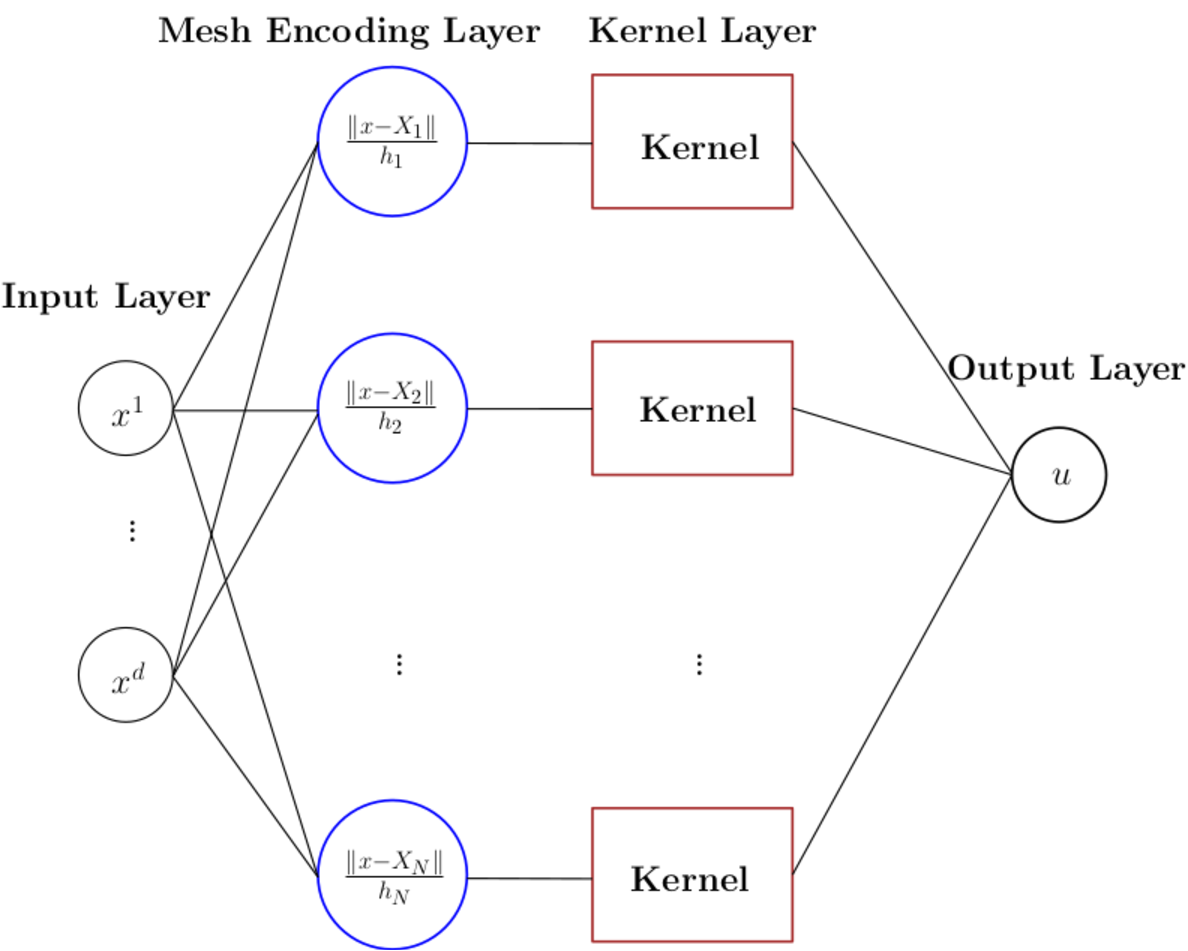
\includegraphics[width=\textwidth]{images/SPINN.pdf}
\caption{Simplified SPINN architecture.}
\label{fig:meshless_nn_repr}
\end{subfigure}
~
\begin{subfigure}{0.4\textwidth}
\centering
\includegraphics[width=\textwidth]{images/softplus_hat_nn.pdf}
\caption{Softplus hat kernel represented as a neural network.}
\label{fig:softplus_hat_nn}
\end{subfigure}
\begin{center}
\begin{subfigure}{0.5\textwidth}
\centering
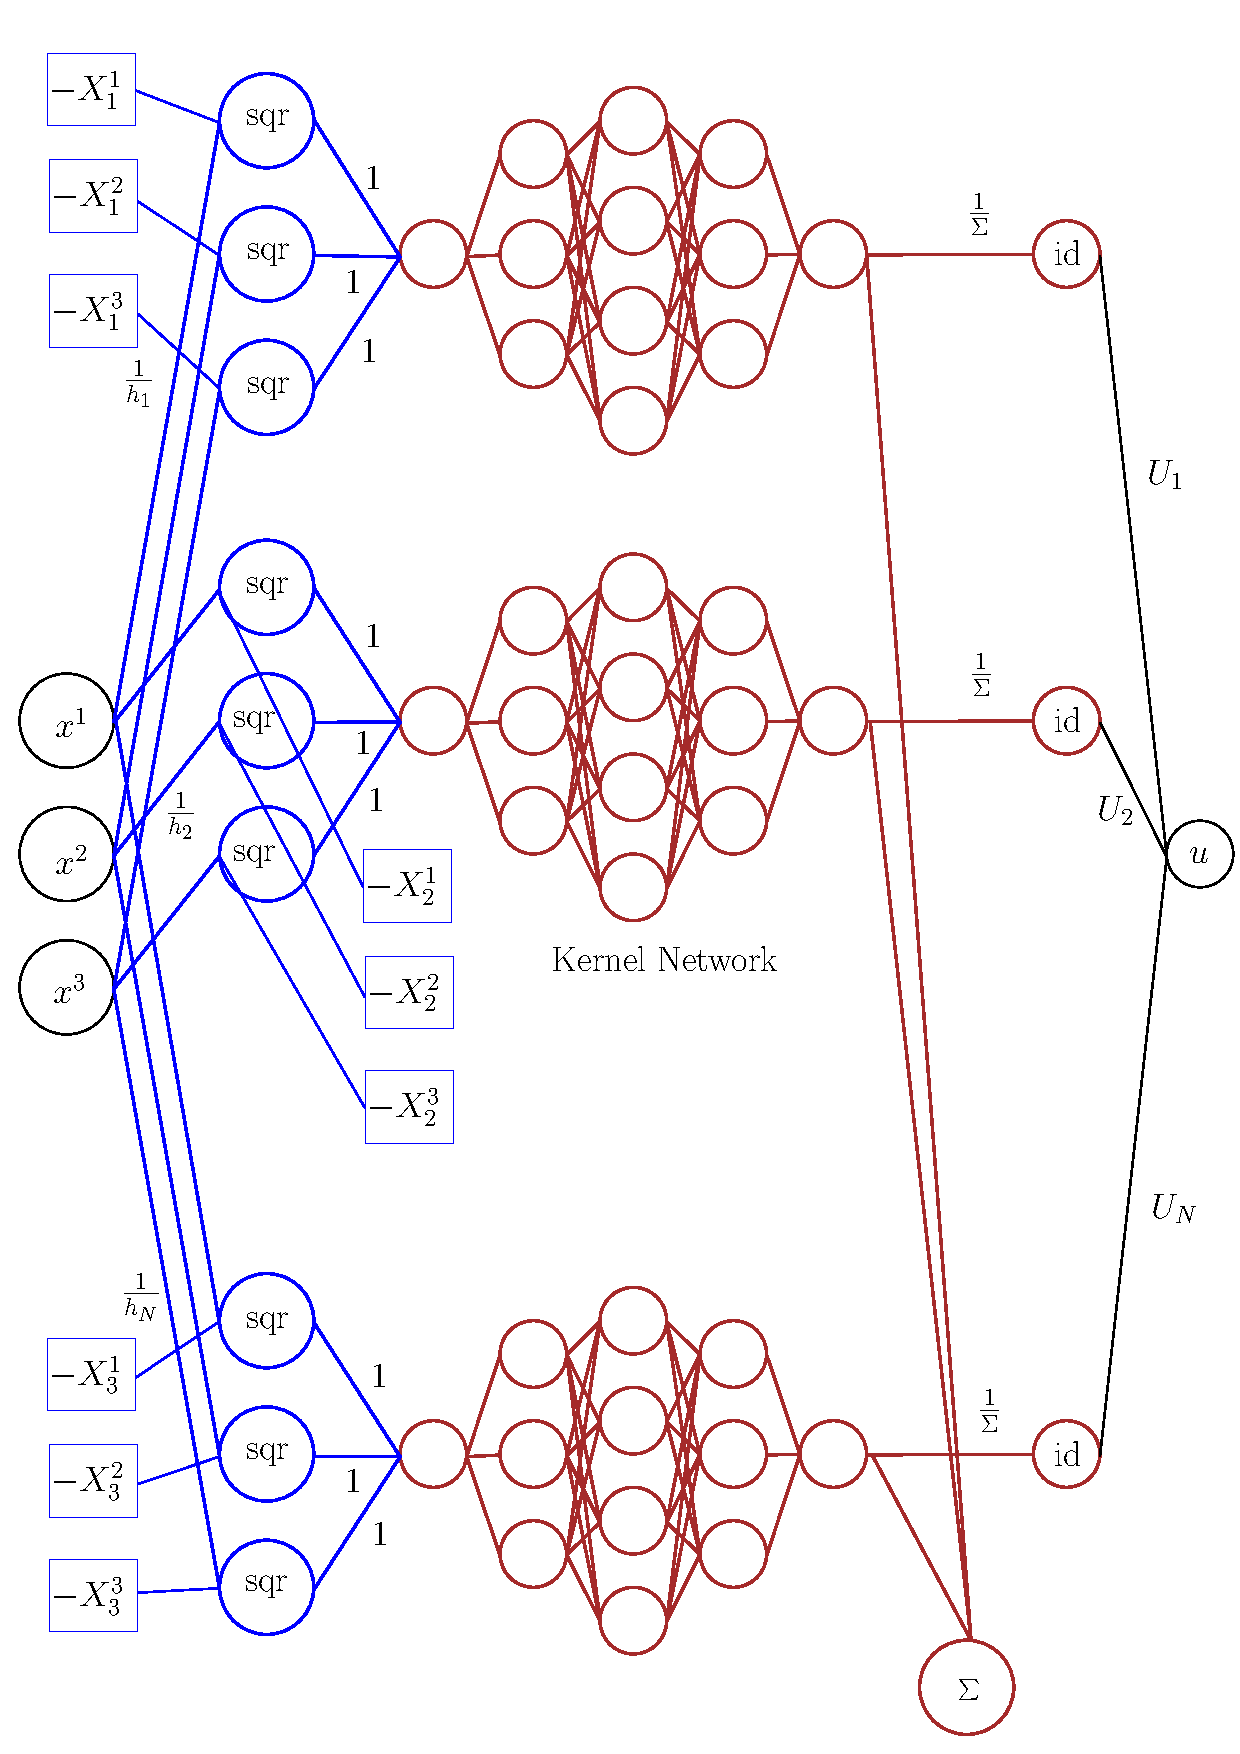
\includegraphics[width=\textwidth]{images/SPINN_detailed.pdf}
\caption{A detailed view of SPINN with DNN kernel.}
\label{fig:meshless_nn_detailed}
\end{subfigure}
\end{center}
\caption{Schematic of SPINN architecture. \ref{fig:meshless_nn_repr} shows the general structure of SPINN as consisting of a mesh encoding layer, followed by a kernel layer. \ref{fig:meshless_nn_detailed} shows a detailed view of a partition of unity SPINN with a deep neural network as its RBF kernel. \ref{fig:softplus_hat_nn} shows how the 2D softplus hat kernel can be recast as a neural network with softplus activation function.}
\label{fig:spinn_architecture}
\end{figure}

\textbf{SPINN architecture.} The foregoing discussion naturally motivates the introduction of generalized meshless approximations where the kernel is represented using a DNN. For instance, a partition of unity meshless approximation of the form \eqref{eq:pde_meshless_PoU} with the kernel replaced by a DNN is shown in Figure~\ref{fig:meshless_nn_detailed}. It can be seen that the mesh encoding layers, shown in blue in Figure~\ref{fig:meshless_nn_detailed}, are identical to that described earlier in the context of the DNN equivalent of \eqref{eq:pde_meshless_approx}. The primary difference is that instead of using an RBF kernel as the activation function in the kernel layer, a standard DNN with any differentiable activation function, shown in brown in Figure~\ref{fig:meshless_nn_detailed}, is used as the kernel; we call this the \emph{kernel network} in the sequel. It is worth pointing out that the \emph{same} kernel network is used for each of the outputs of the mesh encoding layer, in conformity with the meshless ansatz \eqref{eq:pde_meshless_PoU}. We note that the resulting SPINN architecture enjoys the same advantages of the special SPINN architecture introduced earlier: the SPINN architecture proposed here is thus more efficient than conventional DNN based methods such as Deep Ritz \cite{EYu2018}, PINN \cite{RPK2019}, etc. Note also that the number of neurons in the mesh encoding layer is exactly the same as the number of nodes used in the meshless discretization. We thus have a physically inspired means to fix the size of the hidden layers in SPINN, unlike other DNN based approaches like PINN where the size of the hidden layers is arbitrary.  Further, except for the parameters of the kernel network, the remaining learnable parameters of the network are fully interpretable. In fact, once the SPINN model is trained, it is straightforward to extract the corresponding meshless ansatz. The parameters of the kernel network do not require to be interpreted since the kernel network itself can be thought of as a generalized RBF kernel.  

The restriction that the kernel is a radial basis function can be easily removed. It is well known \cite{HLXZ2020} that one-dimensional piecewise linear finite element basis functions can be written exactly in terms of the ReLU basis functions; details are provided in Appendix~\ref{app:relu_fem_1d}. However, ReLU functions are not differentiable, and this can pose problems for their use in ODEs and PDEs of order two or higher. Motivated by the connection between RELU activation functions and hat functions, we propose a new class of basis functions that are infinitely differentiable. We note first that the softplus function
\begin{equation} \label{eq:softplus}
\rho(x) = \log (1 + \exp x),
\end{equation}
provides a smooth approximation of the ReLU function. It is then straightforward to see that the function
\begin{equation} \label{eq:hat_softplus_1d}
N(x) = \frac{1}{\rho(1)}\rho\left(1 + 2\log 2 - \rho(x) - \rho(-x)\right)
\end{equation}
is a function which resembles kernels used in meshless approximations; we call this the \emph{softplus hat kernel}. The constants are chosen such that $N(0) = 1$. Crucially though, the softplus hat kernel \eqref{eq:hat_softplus_1d} is representable as a two layer neural network with softplus activation function; the relevant details are provided in Appendix B. It is also straightforward to generalize this to higher dimensions. For instance, a $d$ dimensional softplus hat kernel is given by
\begin{equation} \label{eq:hat_softplus_nd}
N(x^1, \ldots, x^d) = \frac{1}{\rho(1)}\rho\left(1 + 2d\log 2 - \sum_{k=1}^d (\rho(x^i) + \rho(-x^i))\right).
\end{equation}
We emphasize that the higher dimensional softplus hat kernel functions \eqref{eq:hat_softplus_nd} are also representable directly as a two layer neural network; this is illustrated for two dimensional softplus hat kernels in Figure~\ref{fig:softplus_hat_nn}. We wish to point that the softplus hat kernel is new and has not been used before to the best of the our knowledge. With the choice of these softplus hat kernel functions, meshless approximations that go beyond radial basis functions are constructed along the same lines mentioned before. We present many examples using these softplus hat kernels in the Results section.

\textbf{Mesh adaptivity.} We wish to highlight the fact that since the positions of the nodes and the widths of the kernel associated with the nodes are trainable parameters of the network, the learning algorithm implicitly encodes mesh adaptivity as part of the training process. We note in particular that for problems with large gradients, the widths of the kernels naturally develop a multiscale hierarchy during training.

\textbf{Loss definition.} With this choice of architecture, solving the PDE, $\mathcal{N}(x, u, \nabla u, \ldots) = 0$, is easily accomplished using a collocation technique similar to the one used in PINNs \cite{RPK2019}. We also note in passing that for PDEs that are obtained as the Euler-Lagrange equations of a known functional, the loss function can be formulated using quadratures of the integral of the functional along with penalty terms to enforce boundary conditions, as is carried out in the Deep Ritz method \cite{EYu2018}.

\textbf{Time dependent PDEs.} There are two different approaches for time dependent PDEs using SPINN. The first employs a space-time grid of dimension $d + 1$ and uses exactly the same ideas presented above to solve a time dependent PDE. Alternatively, a hybrid finite difference and SPINN method, whihc we call FD-SPINN, can be employed which performs time marching using conventional finite difference methods and performs spatial discretization at each time step using the SPINN architecture. It is worth mentioning that both explicit and implicit finite difference schemes are subsumed in FD-SPINN. Both the space-time and the FD-SPINN methods are illustrated later on. 


\textbf{Fourier-SPINN.} Another generalization that is naturally suggested by the SPINN architecture is a DNN analogue of familiar decompositions like the Fourier and wavelet transforms. To make this precise, consider the Fourier expansion of a function $u:[a,b] \to \mathbb{R}$, namely $u(x) = a_0 + \sum_{k=1}^{\infty} a_k \cos k\omega x + \sum_{k=1}^{\infty} b_k \sin k\omega x$, where $\omega = 2\pi/(b - a)$. It is straightforward to reinterpret this as a neural network with one hidden layer that has the sinusoidal functions as the activation functions of the neurons. The weights and biases of this neural network are fully interpretable as in the case of the meshless approximation discussed earlier; more details are presented in Appendix~\ref{app:fourier_spinn}. We note in passing that wavelet transforms could also be represented using SPINN. As a natural generalization one could replace the sinusoidal functions by a DNN thereby providing a neural network generalization of the Fourier transform.  

\section*{Results}
We now present solutions of a variety of ordinary and partial differential equations using SPINN. We implement the SPINN architecture using PyTorch~\cite{pytorch}, and the code is available at \url{https://github.com/nn4pde/SPINN}. All our results are automated using \code{automan}~\cite{automan:2018} for easy reproducibility.

\textbf{Ordinary differential equations.} To validate the SPINN method, we first consider ordinary differential equations (ODEs) with different boundary conditions. Sample results are shown in Figure~\ref{fig:spinn_ode} for ODEs with both Dirichlet and Neumann boundary conditions; more examples and details of the various simulations are provided in Appendix~\ref{app:ode}. In Figure~\ref{fig:ode3_gaussian_n_3_comp} we present solutions of the ODE $u''(x) + x(\exp (-(x - (1/3))^2/K) - \exp (-4/9K)) = 0$, $x \in (0,1)$, with zero Dirichlet boundary conditions at $x=0$ and $x=1$ using three different SPINN variants - SPINN with Gaussian kernel and strong form collocation as loss function, variational version of SPINN with Gaussian kernel minimizing the loss functional $I(u) = \int_0^1 (1/2)(u'(x))^2 - f(x)\, dx$, and Fourier-SPINN. The positions of the nodes learnt by the SPINN algorithm are also shown. It is worth pointing out that the nodes adapt to the solution as part of the training process. For the rest of the plots in Figure~\ref{fig:spinn_ode}, strong form based collocation is used. The convergence of SPINN solutions with a fixed number of nodes but different kernels, as a function of the iteration number, is shown in Figure~\ref{fig:ode3_Linf_n_3}. Gaussian, softplus hat and a DNN with two hidden layers of 5 neurons each are used as the kernels. For all the kernels, it is observed that the error plot shows two distinct regimes. Examining the intermediate solutions during the iteration reveals that the first phase in Figure~\ref{fig:ode3_Linf_n_3} characterized by high loss and slow convergence correlates with the SPINN model minimizing the interior loss. The second phase in Figure~\ref{fig:ode3_Linf_n_3} characterized by a rapid drop in the error correlates with the SPINN model learning the boundary conditions of the ODE. It is further seen that all three kernels perform well, though the Gaussian kernel performs well for this ODE. In obtaining the results in Figure~\ref{fig:ode3_gaussian_n_3_comp} and Figure~\ref{fig:ode3_Linf_n_3}, full sampling is used. 

We present next a solution of the ODE $u''(x) + \pi^2 u(x) = \pi \sin \pi x$, $x \in (0,1)$, with $u(0) = 0$ and $u'(1) = 1/2$. To handle the Neumann boundary condition at $x=1$, no fixed node is used there and the interior nodes are free to move outside the domain to accommodate the Neumann condition. This is indeed seen in the SPINN solution shown in Figure~\ref{fig:ode2_n_5_f_0p2} where two of the five interior nodes have moved outside the domain $(0,1)$ during the training. When computing the loss, using full sampling does not work in this case as the SPINN algorithm gets trapped in a metastable state which corresponds to an incorrect solution. Random sampling of the interior points, however, provides a convenient means for the SPINN algorithm to escape this metastable state and learn the correct solution. We illustrate the effect of sampling ratio $f$ on the convergence of the SPINN algorithm in Figure~\ref{fig:ode2_n_5_Linf}, thereby demonstrating the significant effect that random sampling has on the convergence of the algorithm for this ODE.

\begin{figure}[htpb]
\begin{subfigure}{0.5\textwidth}
\centering
\includegraphics[width=\textwidth]{figures/ode3_comp/ode3_comp.pdf}
\caption{ODE with Dirichlet boundary conditions.}
\label{fig:ode3_gaussian_n_3_comp}
\end{subfigure}
~
\begin{subfigure}{0.5\textwidth}
\centering
\includegraphics[width=\textwidth]{figures/ode3_conv_3/ode3_Linf_error_n_3.pdf}
\caption{$L_{\infty}$ error for different kernels.}
\label{fig:ode3_Linf_n_3}  
\end{subfigure}

\begin{subfigure}{0.5\textwidth}
\centering
\includegraphics[width=\textwidth]{figures/ode2_conv_5/ode2_n_5_f_0.2.pdf}
\caption{ODE with Neumann boundary condition and random sampling.}
\label{fig:ode2_n_5_f_0p2} 
\end{subfigure}
~
\begin{subfigure}{0.5\textwidth}
\centering
\includegraphics[width=\textwidth]{figures/ode2_conv_5/ode2_Linf_error_n_5_f.pdf}
\caption{$L_{\infty}$ error for different sampling fractions.}
\label{fig:ode2_n_5_Linf}    
\end{subfigure}
\caption{Solution of ODEs with SPINN. \ref{fig:ode3_gaussian_n_3} shows the solution of the ODE $u''(x) + f(x) = 0$, $x \in (0,1)$, $u(0) = u(1) = 0$, where $f(x) = x(\exp (-(x - (1/3))^2/K) - \exp (-4/9K))$ computed using SPINN with Gaussian kernel. The positions of the nodes learnt by SPINN is shown as blue dots. The $L_{\infty}$ error associated with different choices of kernels is shown in \ref{fig:ode3_Linf_n_3}. The solution of the ODE $u''(x) + \pi^2 u(x) = \pi \sin \pi x$, $x \in (0,1)$, with $u(0) = 0$ and $u'(1) = 1/2$ is shown in \ref{fig:ode2_n_5_f_0p2}. A random sampling fraction $f=0.2$ is used in this case. The $L_{\infty}$ errors for different sampling fractions are shown in \ref{fig:ode2_n_5_Linf}.}
\label{fig:spinn_ode}
\end{figure}

\textbf{PDEs in two dimensions.}
We now present a few examples solving PDEs, specifically the Poisson equation in two dimensions. The first example solves the equation $\nabla^2 u(x, y) = 20\pi^2 \sin 2\pi x \, \sin 4 \pi y$ on the unit square $[0,1]\times[0,1]$ with zero Dirichlet boundary conditions. A comparison of the SPINN solution with the exact solution is shown in Figure~\ref{fig:2d_A_softplus_n_100}. The $L_{\infty}$ error as a function of the iteration number is plotted for different kernels in Figure~\ref{fig:2d_A_Linf_n_100}. The kernels chosen here are identical to those considered earlier in the one dimensional case. As before, we observe two distinct regimes in the error graph corresponding to learning the interior and learning the boundary conditions. While all three kernels provide a good solution, the softplus hat kernel performs better than the other two for this PDE. The convergence of the SPINN solution as a function of the number of interior nodes used is shown in Figure~\ref{fig:2d_A_Linf}; we observe that the error decreases with increase in the number of nodes, as expected. 

For the second example we consider $\nabla^2 u(x, y) + 1 = 0$ on the domain $[-1,1]\times[-1,1] \setminus [0,1]\times\{0\}$. The solution obtained using SPINN is shown in Figure~\ref{fig:poisson_2d_square_slit_sol}. The corresponding nodal positions are shown in Figure~\ref{fig:poisson_2d_square_slit_nodes}. It is seen that the SPINN algorithm learns the optimal position of the nodes and the size of the kernels at the nodal positions appropriately. A comparison of the error of the SPINN solution with respect to a reference finite element solution using a very fine mesh is shown in Figure~\ref{fig:poisson_2d_square_slit_convergence}. 

The examples shown so far feature domains with regular geometric shapes. The SPINN algorithm, however, works well on arbitrarily shaped domains too. The solution of the Poisson equation $\nabla^2 u(x,y) + 1 = 0$ on an irregularly shaped domain is shown in Figure~\ref{fig:poisson2d_irregular}, and a reference finite element solution computed using a fine mesh is shown in Figure~\ref{fig:poisson2d_irregular_fem}. The distribution of the nodes in this case is shown in Figure~\ref{fig:poisson2d_irregular_nodes}.  The $L_{\infty}$ error of the SPINN solution was found to be around $4.9\times 10^{-3}$. 

\begin{figure}
\begin{subfigure}{0.32\textwidth}
\centering
\includegraphics[width=\textwidth]{figures/poisson2d_sine_conv/sine2d_softplus_n_100.pdf}
\caption{SPINN solution with softplus hat kernel.}
\label{fig:2d_A_softplus_n_100}    
\end{subfigure}
~
\begin{subfigure}{0.32\textwidth}
\centering
\includegraphics[width=\textwidth]{figures/poisson2d_sine_conv/sine2d_Linf_error_n_100.pdf}
\caption{$L_{\infty}$ error as a function of iteration.}
\label{fig:2d_A_Linf_n_100}      
\end{subfigure}
~
\begin{subfigure}{0.32\textwidth}
\centering
\includegraphics[width=\textwidth]{figures/poisson2d_sine_nodes/sine2d_Linf_error.pdf}
\caption{$L_{\infty}$ error as a function of number of internal nodes.}
\label{fig:2d_A_Linf}
\end{subfigure}

\begin{subfigure}{0.32\textwidth}
\includegraphics[width=\textwidth]{figures/square_slit/solution.png}
\caption{SPINN solution of the square slit problem.}
\label{fig:poisson_2d_square_slit_sol}
\end{subfigure}
~
\begin{subfigure}{0.32\textwidth}
\includegraphics[width=\textwidth]{figures/square_slit/sol_centers.png}
\caption{Node and kernel width distribution.}
\label{fig:poisson_2d_square_slit_nodes}
\end{subfigure}
~
\begin{subfigure}{0.32\textwidth}
\includegraphics[width=\textwidth]{figures/square_slit/square_slit_Linf_error.pdf}
\caption{$L_{\infty}$ error as function of number of internal nodes.}
\label{fig:poisson_2d_square_slit_convergence}
\end{subfigure}

\begin{subfigure}{0.32\textwidth}
\centering
\includegraphics[width=\textwidth]{figures/irregular/spinn_solution.png}
\caption{Poisson equation on irregular domain.}
\label{fig:poisson2d_irregular}
\end{subfigure}
~
\begin{subfigure}{0.32\textwidth}
\includegraphics[width=\textwidth]{figures/irregular/sol_centers.png}
\caption{Node and kernel width distribution.}
\label{fig:poisson2d_irregular_nodes}
\end{subfigure}
~
\begin{subfigure}{0.32\textwidth}
\includegraphics[width=\textwidth]{figures/irregular/fem_solution.png}
\caption{Reference FEM solution}
\label{fig:poisson2d_irregular_fem}
\end{subfigure}
\caption{SPINN solutions for PDEs in two dimensions.  Figures~\ref{fig:2d_A_softplus_n_100}, \ref{fig:poisson_2d_square_slit_sol}, \ref{fig:poisson2d_irregular} represent the SPINN solution for three different PDEs; see text for details. The node and kernel width distributions for the solutions learnt by SPINN are shown in Figures~\ref{fig:poisson_2d_square_slit_nodes}, \ref{fig:poisson2d_irregular_nodes}. Various convergence plots for the SPINN solutions obtained are shown in Figures~\ref{fig:2d_A_Linf_n_100}, ~\ref{fig:2d_A_Linf},  ~\ref{fig:poisson_2d_square_slit_convergence}.}
\label{fig:spinn_pde2d}
\end{figure}

\textbf{Heat equation.}
We now present examples involving time dependent PDEs. To start with, we consider the one-dimensional heat equation $u_t = c^2 u_{xx}$, where $x \in (0,1)$ and $t \in [0, T]$. We consider two different methods to solve the heat equation. First, we solve it using the implicit FD-SPINN algorithm $u^{n+1} = u^n + c^2 \Delta t \, u^{n+1}_{xx}$. We show time snapshots of the solution in Figure~\ref{fig:heat_eqn_compare}. We also solve this problem as a space-time PDE by emplying SPINN to simultaneously approximate the solution in space and time. The solution is compared with the exact solution in Figure~\ref{fig:heat_eqn_compare} and the space-time solution is shown in Figure~\ref{fig:heat_eqn_st_sol}; the exact solution is also shown as a wireframe for comparison.

\begin{figure}
\begin{subfigure}{0.32\textwidth}
\includegraphics[width=\textwidth]{figures/burgers_fd/gaussian_n40.pdf}
\caption{FD-SPINN of Burgers' equation compared with reference PyClaw solution.}
\label{fig:burgers_comp}
\end{subfigure}
~
\begin{subfigure}{0.32\textwidth}
\includegraphics[width=\textwidth]{figures/heat/u_compare.pdf}
\caption{Comparison of exact and SPINN solutions of the heat equation.}
\label{fig:heat_eqn_compare}
\end{subfigure}
~
\begin{subfigure}{0.32\textwidth}
\includegraphics[width=\textwidth]{figures/heat/st_sol.png}
\caption{Space-time solution of the heat equation.}
\label{fig:heat_eqn_st_sol}
\end{subfigure}

\begin{subfigure}{0.32\textwidth}
\includegraphics[width=\textwidth]{figures/advection/u_compare.pdf}
\caption{Comparison of exact and SPINN solutions for advection equation.}
\label{fig:advection_comp}
\end{subfigure}
~
\begin{subfigure}{0.32\textwidth}
\includegraphics[width=\textwidth]{figures/advection/st_sol.png}
\caption{Space-time solution of advection equation.}
\label{fig:advection_st}
\end{subfigure}
~
\begin{subfigure}{0.32\textwidth}
\includegraphics[scale=0.2]{figures/advection/sol_centers.png}
\caption{Node and kernel width distributions for advection equation.}
\label{fig:advection_nodes}
\end{subfigure}
\caption{Figure~\ref{fig:heat_eqn_compare} compares the heat equation solution on the domain $(0,1)$ over time interval $[0, 0.2]$ using the implicit finite difference SPINN, the space-time solution, and exact solution. Figure~\ref{fig:heat_eqn_st_sol} depicts the space time solution for the heat equation.  Figure~\ref{fig:advection_comp} shows the solution of the linear advection equation with the hybrid implicit finite difference SPINN, and space-time solution which is also shown in ~\ref{fig:advection_st}.  Figure~\ref{fig:advection_nodes} shows the location of the nodes at different times for the advection problem along with their widths.
Figure~\ref{fig:burgers_comp} depicts the solution of the implicit finite difference SPINN solution for the Burgers' equation and compares it with that obtained using PyClaw.}
\label{fig:time_varying}
\end{figure} 

\textbf{Linear advection equation.}
We study next the classic hyperbolic time-dependent PDE in one spatial dimension, namely the linear advection equation $u_t + au_x = 0$, where $x\in \mathbb{R}$ and $t\in [0, T]$.  The exact solution for this problem with  initial condition $u(x, t=0) = u_0(x)$ is $u(x, t) = u_0(x - at)$. As done earlier for the heat equation, we solve the problem using both a first-order, implicit FD-SPINN as well as a space-time SPINN.  Time snapshots of the solution with a Gaussian pulse as initial condition are shown in Figure~\ref{fig:advection_comp}.  In Figure~\ref{fig:advection_st} the space-time solution is compared with the exact solution, shown in wireframe.  The location of the interior nodes along with the kernel widths is shown in Figure~\ref{fig:advection_nodes}.  The nodes are initially placed uniformly. It is worth emphasizing that the nodes adapt in time and space to capture the features of the solution, which in this case is a travelling wave.  We also point out that widths of the kernel are narrow around the peak of the wave while they are broad away from the peak thereby demonstrating mesh-adaptivity.


\textbf{Burgers' equation.}
We next consider a classic non-linear, time-dependent hyperbolic PDE in one spatial dimension, namely the inviscid Burgers' equation $u_t + u u_x = 0$, where $x\in (0, 1)$ and $t\in [0, T]$ with zero Dirichlet boundary conditions and $u(x, t=0) = \sin(2\pi x)$ as the initial condition.  We solve the problem using the FD-SPIN method using 40 internal nodes.  Time snapshots of the solution at different times are shown in Fig.~\ref{fig:burgers_comp}  and compared against reference solution obtained using PyClaw~\cite{pyclaw}.  A shock develops at $x=0$ at around 0.25 seconds which is clearly captured well by the method.  What is remarkable is that despite using smooth kernels, in this case the Gaussian, the FD-SPINN method is able to capture the shock accurately.  This also demonstrates the adaptivity of the SPINN method; the nodes closer to the shock front have a much smaller kernel width in comparison to nodes away from the shock as expected.  This also demonstrates the ability of SPINN to capture discontinuities in the solution.

\textbf{Fluid dynamics.}
Our final example involves solving the steady incompressible viscous Navier-Stokes equations in two spatial dimensions.  We consider the classic lid-driven cavity problem~\cite{ldc:ghia}, wherein a viscous incompressible fluid is contained in a unit square cavity, with the top surface (lid) of the cavity moving at a constant horizontal velocity $u=1$.   The walls are modeled with no-slip boundary conditions consistent with the behavior of a viscous fluid.  The $x$-momentum equation is $u u_x + v u_y + p_x - \nu \nabla^2 u = 0$, and the $y$-momentum equation is $u v_x + v v_y + p_y - \nu \nabla^2 v = 0$, where $(u, v)$ are the components of the velocity,  $p$ is the  pressure, and $\nu$ is the kinematic viscosity of the fluid. The fluid is incompressible and satisfies $u_x + v_y = 0$.  On the walls, we also apply a Neumann boundary condition of $\nabla p \cdot n = 0$, where $n$ is the normal vector at the wall. The magnitude of the velocity computed using SPINN is shown in Fig.~\ref{fig:ldc_velocity}.  In Fig.~\ref{fig:ldc_ghia_compare} the velocity profile along the center-lines are compared with those of \cite{ldc:ghia} as the number of internal nodes is varied.  We obtain good results with around 225 internal nodes for this problem.  This example was chosen to demonstrate the ability of SPINN to model a non-linear system of PDEs that frequently arise in the modeling physical systems.

\begin{figure}
\begin{subfigure}{0.51\textwidth}
\includegraphics[width=\textwidth]{figures/cavity/vmag_n324.pdf}
\caption{Velocity magnitude of flow.}
\label{fig:ldc_velocity}
\end{subfigure}
~
\begin{subfigure}{0.49\textwidth}
\includegraphics[width=\textwidth]{figures/cavity/centerline_compare.pdf}
\caption{Centerline velocity comparison with \cite{ldc:ghia}.}
\label{fig:ldc_ghia_compare}
\end{subfigure}
\caption{Solution of the steady NS equations for the lid-driven cavity problem with a fluid having kinematic viscosity $\nu=0.01$ using SPINN with a Gaussian kernel. On the left the velocity magnitude of the fluid is shown for a case with 324 internal nodes.  On the right we compare the centerline velocity with the standard computational results of \cite{ldc:ghia} as the number of internal nodes is varied.}
\label{fig:ldc}
\end{figure}

\section*{Discussion}

The primary purpose of the various examples presented earlier is to provide a proof-of-concept demonstration that the SPINN model works well for a large class of ODEs and PDEs. There are however many aspects which can be improved. We discuss some of these here; we will be investigating these in forthcoming publications.

\textbf{Boundary conditions.} For all the variants of SPINN presented in this work, the loss is defined as a weighted sum of the interior and boundary losses. The boundary loss, in particular, is enforced as a penalty term that is proportional to the square of the predicted and imposed boundary values. The constant of proportionality, however, is arbitrarily chosen and varies for each problem. This is a well known limitation of penalty based techniques to enforce constraints. While Dirichlet boundary conditions are relatively easy to enforce, capturing Neumann boundary conditions require careful choice of the fixed and free nodes. For instance, a fixed node at a Neumann boundary when using Gaussian kernels will lead to an infinite indeterminacy of the corresponding coefficient since the slope of the Gaussian kernel is zero at its center. This translates to convergence issues with the loss minimization algorithm. As a simple solution, we use fixed nodes only on the Dirichlet boundaries. We observe that the nodes at times move outside the domain to enforce the boundary condition properly. However, we point out that there are other means to enforce boundary conditions like having a fixed layer of nodes along the boundary, as is done in some particle based methods like Smoothed Particle Hydrodynamics (SPH)~\cite{ye2019sph}.

\textbf{Time dependent PDEs with spacetime SPINN.} The handling of time dependent partial differential equations using the space-time version of SPINN poses a few challenges. While it is possible to treat a time dependent PDE defined on a $d$ dimensional domain as a PDE on $d + 1$ dimensional space-time domain, this can fail to capture certain phenomena like shocks satisfactorily. To explain this further, considering the case of a shock in a hyperbolic PDE, the region ahead of the shock has no information about the region behind it. However, when using a space-time SPINN model, the kernels \emph{extend} isotropically into both the space and time directions. This often results in an artificial smoothness in the SPINN solution that doesn't agree with the true solution. We indeed observe this problem when using the space-time SPINN model to solve the Burgers' equation. What is interesting to note is that we observe sharpening of the wave to produce a shock like structure even with the space-time SPINN model, but the isotropic extension of the kernels along future and past times alike results in a smoothed solution that is more dissipative than the actual solution. A possible amelioration is to use time-asymmetric kernels, which are in principle describable using custom or DNN kernels.

On the other hand, the FD-SPINN algorithm does not suffer from this problem since SPINN is only used to represent the spatial solution and the problem is still asymmetric in time owing to the use of finite differences to approximate time derivatives. While we have used a first order scheme here as proof-of-concept of FD-SPINN, it is in principle straightforward to implement higher order schemes to control the time discretization errors using methods such as those proposed in \cite{SCL2020pre}. We also point out that the FD-SPINN algorithms presented here are different from the corresponding finite difference schemes since the spatial derivatives are handled \emph{exactly} using automatic differentiation. Automatic differentiation has been used in the context of finite element discretization problems in both static \cite{TRRB2002} and dynamic \cite{RG2014} PDEs, but the implicit finite difference schemes we propose here provide a systematic means to develop a variety of efficient time marching schemes.

\textbf{Computational efficiency.} The current implementation of SPINN has been designed as a proof-of-concept.  While the problems considered in this work can be solved with very little computational effort, the implementation will not scale well for larger problems. This is because the method currently evaluates the effect of \emph{all} the nodes on a given sample point making the problem $O(NM)$ given $N$ nodes and $M$ samples.  We have investigated performing spatial convolutions using the \texttt{pytorch-geometric} package~\cite{pytorch_geometric} to accelerate this computation by restricting the interaction of sampling points only with their nearest nodes, thereby reducing the problem to $O(nM)$ where $n$ is the typical number of neighbors.  While preliminary results are encouraging and allow us to use more nodes, there are some limitations and constraints that need to be investigated further. 

\textbf{Wavelet transforms.} The results presented earlier highlight how the SPINN model is able to learn a variety of different length and time scales inherent in a given problem as part of the learning algorithm. A class of classical computational models for multiresolution analysis is wavelet based solutions of PDEs; see for instance \cite{WA94}. It is straightforward to recast wavelet transforms as a SPINN architecture in a manner similar to how the Fourier transform are handled in this work. An advantage of wavelet based representations is that the structure inherent in the scaling and shifting operations in wavelets can be efficiently implemented using spatial convolutions discussed earlier. We wish to reiterate that our current SPINN model already possesses a multiresolution capability on account of the kernel centers and widths being trainable parameters, as is amply demonstrated in the various examples presented.


\textbf{Finite element based extensions of SPINN.} We have used meshless approximations to motivate the development of the SPINN architecture in this work. However, conforming mesh based representations like finite elements could also be used to develop the corresponding neural network generalizations, although the connection is not straightforward. The difficulty arises because of the fact that enforcing mesh conformity places more constraints on the architecture. There are theoretical results elaborating the relation between finite element models and DNNs. For instance in \cite{HLXZ2020} the authors show how every piecewise linear finite element model can be mapped to a ReLU DNN, while in \cite{OPS19} higher order finite elements have been investigated along similar lines.  The advantage in using meshless representations over conforming mesh representations based on the finite elements is that the corresponding DNN has more flexibility in how the nodes move, and how the kernel widths adapt. In addition it also allows for a variety of generalizations like the Fourier and wavelet generalizations of SPINN.

\textbf{Interpreting deep neural network solutions of PDEs.} An interesting consequence of the methodology we present here to reinterpret meshless methods as sparse DNNs is that it also provides a means to interpret certain DNNs such as PINNs~\cite{RPK2019}. Specifically, a DNN approximation of a function $u:\mathbb{R}^d \to \mathbb{R}$ consisting of $N$ hidden layers with $(n_1, n_2, \ldots, n_N)$ neurons in each layer can be thought of as a global approximation of $u$ over its domain in terms of $n_N$ basis functions. If $\sigma$ denotes the activation function of the PINN and $h_k$ denotes the linear function relating the $(k-1)^{\text{th}}$ hidden layer to the $k^{\text{th}}$ hidden layer, $k = 1, \ldots, N$, with $k = 0$ denoting the input layer and $k = N + 1$ denoting the output layer, then it follows immediately from the structure of the network that
\begin{displaymath}
u(x) = w_0 + \sum_{i=1}^{n_N} w_i \,(\sigma \circ h_{N} \circ \sigma \circ h_{N-1} \circ \ldots \circ h_1)_i(x).
\end{displaymath}
Thus denoting by $\phi_i$ the output of the $i^{th}$ neuron in the last hidden layer, we see that the PINN approximation can be written as
\begin{displaymath}
u(x) = w_0 + \sum_{i=1}^{n_N} w_i \phi_i(x).
\end{displaymath}
We thus see that the final layer connection weights and biases can be interpreted as the coefficients of a Ritz type approximation of $u$. Thus using a collocation technique to train the network as is done in PINNs can be thought of as learning global basis functions and their corresponding weights, with the caveat that different nodes have different basis functions. SPINNs, on the other hand are more efficient since they use shifted and scaled versions of a single kernel. They can thus be thought of as an improvement of PINNs by using known information about basis functions to sparsify the network structure and eliminate the arbitrariness that attends the choice of DNN architectures in PINNs.  


\section*{Conclusion}
To conclude, we have presented a new class of sparse DNNs which we call SPINN - Sparse, Physics-based and Interpretable Neural Networks - which naturally generalize classical meshless methods while retaining the advantages of DNNs. The key features  of SPINN are (i) it is fully interpretable in sharp contrast to DNNs, (ii) it is efficient in comparison with a DNN with the same number of neurons on account of its sparsity, (iii) it is physics-based since the loss function depends directly on the strong form of a PDE or its variational form, and (iv) it suggests new avenues of research like Fourier and wavelet based architectures. We have demonstrated this using a variety of ODEs and PDEs in this work.  We thus envisage SPINN as a novel numerical method that seamlessly bridges traditional meshless methods and modern DNN-based algorithms for solving PDEs.  Recognizing this link opens the door for developing new numerical algorithms that blend the best of both worlds. Finally, even a mere re-expression of meshless algorithms as a SPINN model makes it easier to enhancing traditional meshless methods along the lines of differentiable programming.

\section*{Methods}
The SPINN architecture proposed in this work is easily implementable using standard NN libraries. We provide PyTorch implementations of all the examples considered in this work at \url{https://github.com/nn4pde/SPINN}.

We present here certain details of the implementation. We classify the nodes associated with the SPINN model as fixed and free nodes. Fixed nodes are typically used on the (Dirichlet) boundaries. Free nodes, on the other hand, are used inside the domain of definition of the problem. Both fixed and free nodes are designed to have variable kernel widths, but the free nodes are also free to move both inside and outside the domain. A separate set of sampling points on the interior and boundary of the domain are also used. These are the points where the interior and boundary losses are evaluated using the SPINN model. We provide options for both full sampling and random sampling. In random sampling, a random subset of an initially generated set of sampling points is chosen for each iteration of the loss minimization algorithm. The output layer weights and biases are set to zero by default. This implies in particular that when using full sampling and either the Gaussian or softplus hat kernels, the SPINN algorithm is fully deterministic. Thus there are only two sources of stochasticity in the current implementation of SPINN: (i) randomness due to initialization of the DNN kernel weights and biases when DNN kernels are used, and (ii) randomness due to sampling of the interior sampling points when random sampling is used. We do not sample on the boundary and use full boundary sampling always. This is because of the fact that boundary conditions are more delicate to impose in the current framework.

To illustrate the loss functions used in training the SPINN models, consider the special case of a second order PDE of the form
\begin{displaymath}
\begin{split}
\mathcal{N}(x, u(x), \nabla u(x), \nabla^2 u(x)) = 0, \quad x \in \Omega,\\
u = u_0 \;\text{ on }\partial_0 \Omega, \quad \nabla u \cdot n = g_0 \;\text{ on } \partial \Omega \setminus \partial_0 \Omega,
\end{split}
\end{displaymath}
where $n$ is the outward unit normal to $\partial \Omega$. The generalization to other ODEs and PDEs is straightforward. The loss function for traing the SPINN network for this problem is chosen as
\begin{equation} \label{eq:spinn_loss}
\begin{split}
L((h_i), (X_i), (U_i)) &= w_i \sum_{i=1}^{M_i} \mathcal{N}(\xi_i, u(\xi_i), \nabla u(\xi_i), \nabla^2 u(\xi_i))\\
 &+ w_d \sum_{i=1}^{M_d} (u(\eta_i) - u_0(\eta_i))^2\\
 &+ w_n \sum_{i=1}^{M_n} \left(\nabla u(\zeta_i)\cdot n(\zeta_i) - g_0(\zeta_i)\right)^2.
\end{split}
\end{equation}
Here $w_i$, $w_d$ and $w_n$ are constants that enforce the loss in the interior of the domain, the Dirichlet boundary, and the Neumann boundary, respectively. The set of points $(\xi_i)_{i=1}^{M_i}$, $(\eta_i)_{i=1}^{M_d}$ and $(\zeta_i)_{i=1}^{M_n}$ in the interior of $\Omega$, and on the Dirichlet and Neumann boundaries on $\Omega$, respectively, are the sampling points where the loss is evaluated. In cases where a variational form
\begin{equation} \label{eq:weak_form}
I(u) = \int_{\Omega} f(x, u(x), \nabla u(x))\,dx
\end{equation}
is available for the PDE, the interior loss can alternatively be defined directly in terms of an appropriate quadrature approximation of the integral in \eqref{eq:weak_form}. Dirichlet boundary conditions are imposed using penalty terms as in the strong form collocation case described earlier. Neumann boundary conditions, on the other hand, are directly integrated into the definition of the integral loss functional. For the ODE example used in the text to illustrate the variational version of SPINN, a simple Riemannian sum computed over a fine partition of the domain of the ODE was used to estimate the integral. The optimization of the SPINN models is carried out using any of the well known optimizers. All the examples presented in this work were carried out using the Adam optimizer \cite{kingma2014} implemented in PyTorch.

For time dependent PDEs we use two different SPINN algorithms. The first is the  FD-SPINN method that uses finite differences to discretize in time and SPINN for the spatial approximation. We illustrate this in the special case of the heat equation, with a similar formalism for the advection and Burgers' equations. Choosing a time step $\Delta t$, we denote by $(u^k(x))_{k=1}^{N_t}$ the approximations to the solution $u(x, k\Delta t)$; here $N_t$ is chosen such that $N_t \Delta t \simeq T$. The following first order implicit time difference scheme is used in this work:
\begin{displaymath}
\frac{u^{n+1}(x) - u^n(x)}{\Delta t} = \frac{d^2 u^{n+1}(x)}{d x^2}, \quad n = 1, \ldots, N_t.
\end{displaymath}
We wish to emphasize that the spatial derivatives are computed \emph{exactly} using automatic differentiation since the spatial approximation uses SPINN. Thus this implicit scheme is different in comparison to traditional time marching schemes. The loss in the interior of the domain $[0,L]$ is computed as the squared residue of the foregoing equation. The second algorithm uses SPINN for both space and time discretization. The implementation of the space-time SPINN solution is similar to the implementation of second order PDEs described earlier.

\section*{Author contributions}
Both authors contributed equally to the conceptualization, formulation of the problem, developing the codes, performing the analyses and writing the manuscript.  

\bibliographystyle{plain}
\bibliography{spinn}

\newpage
\section*{Supplementary Material}
\appendix

\section{ReLU networks and piecewise linear finite element approximation} \label{app:relu_fem_1d}
In this section, we illustrate the connection between SPINN and DNN represenations for PDEs that have been been previously studied. To keep the discussion concrete we focus on the special case of one spatial dimension. Consider the problem of minimizing the functional $I:H^1_0([0,1]) \to \mathbb{R}$, 
\begin{equation} \label{eq:fnl_1d}
I(u) = \frac{1}{2}\int_0^1 \left(\frac{du(x)}{dx}\right)^2 \,dx - \int_0^1 f(x)u(x) \,dx,
\end{equation}
where $f \in L^2([0,1])$. A standard argument shows that the Euler-Lagrange equations corresponding to the minimization of the functional \eqref{eq:fnl_1d} is the second order ODE:
\begin{equation} \label{eq:ode_2ndorder_1d}
\begin{split}
\frac{d^2u(x)}{dx^2} + f(x) = 0, & \quad x \in [0,1],\\
u(0) = 0, & \quad u(1) = 0.
\end{split}
\end{equation}
To illustrate this, we consider the special case of a piecewise linear finite element approximation of the solution of \eqref{eq:ode_2ndorder_1d}. The basis functions for a piecewise linear finite element approximation can be equivalently thought of as ReLU network with one hidden layer. For this case, a convenient SPINN architecture is the following ReLU network with one hidden layer: 
\begin{equation} \label{eq:spinn_1d}
u(x) = \sum_{i=0}^N w_i \text{ReLU}(x - x_i),
\end{equation}
Following \cite{HLXZ2020}, we outline the relation between a piecewise linear finite element representation of a function $u:[a,b] \to \mathbb{R}$ and neural networks with ReLU activation functions. Letting $(x_i)_{i=0}^N$ be a partition of $[a,b]$, such that $x_0 = a$, $x_N = b$, and $x_i < x_{i+1}$ for $0 \le i < N$, the piecewise linear basis function $N_i(x)$, for $1 < i < N$, is given by
\begin{equation} \label{eq:hat_function_fem_1d}
N_i(x) = \begin{cases}
\frac{x_i - x}{x_i - x_{i-1}}, & x \in [x_{i-1},x_i],\\
\frac{x - x_i}{x_{i+1} - x_i}, & x \in [x_i, x_{i+1}].
\end{cases}
\end{equation}
An important observation that connects the finite element approximation of $u$ with ReLU neural networks is the fact that the basis function in \eqref{eq:hat_function_fem_1d} can be written as a linear combination of ReLU functions in the following form:
\begin{equation} \label{eq:hat_1d_relu_repr}
N_i(x) = \frac{1}{h_i}\text{ReLU}(x - x_{i-1}) - \left(\frac{1}{h_i} + \frac{1}{h_{i+1}}\right)\text{ReLU}(x - x_i) + \frac{1}{h_{i+1}}\text{ReLU}(x - x_{i+1}),
\end{equation}
where we use the symbols $h_k = x_{k} - x_{k-1}$, $1 < k < N$, to denote the lengths of the various elements in a given partition of $[a,b]$. Using \eqref{eq:hat_function_fem_1d} and \eqref{eq:hat_1d_relu_repr}, we can write the piecewise linear finite element approximation of $u$, namely
\begin{equation} \label{eq:fem_approx_1d}
u(x) = \sum_{i=0}^N N_i(x) U_i,
\end{equation}
as
\begin{equation} \label{eq:fem_1d_ReLU}
u(x) = \sum_{i=0}^{N - 1} (\theta_{i+1} - \theta_i) \text{ReLU}(x - x_i),
\end{equation}
where $\theta_i = (U_i - U_{i-1})/h_i$. The representation \eqref{eq:fem_1d_ReLU} informs us that a piecewise linear finite element approximation of 1d functions is equivalent to a DNN with one hidden layer with weights and biases consistent with \eqref{eq:fem_1d_ReLU}.

In \cite{HLXZ2020}, the authors proposed a hybrid method wherein they use the representation \eqref{eq:fem_1d_ReLU}, with the weights $(\theta_i)$ computed using the standard finite element method holding the mesh fixed, and the biases $(x_i)$ are computed by minimizing the loss $I$ as a function of the biases $(x_i)$ for fixed values of the weights $(\theta_i)$. This staggered approach, however, does not take full advantage of the variety of stochastic gradient algorithms that have been developed for DNNs. In contrast, the SPINN architecture which we propose in this work does not use a staggered approach, and is more efficient. 

Even in this simple case, we note the following features: (i) the weights connecting the input layer, which just takes in $x$, and the hidden layer is $1$ uniformly, (ii) the biases of the hidden layer are directly interpretable as the position of the nodes of the finite element discretization, and (iii) the weights connecting the hidden layer and the output layer are interpretable in terms of the nodal values of the corresponding finite element solution. We also see that the number of neurons in the hidden layer is just the number of interior nodes in the finite element discretization. This is in sharp contrast to the approach followed in Physics Informed Neural Networks (PINN) \cite{RPK2019}, or the Deep-Ritz method \cite{EYu2018}, which employ dense neural networks, and hence are not easily interpretable. 

\section{Kernel functions} \label{app:softplus}
Motivated by the fact that piecewise linear finite element basis functions in 1D can be written in terms of ReLU functions, we propose a new class of basis functions in one and higher dimensions that naturally generalize ReLU-based shape functions that are differentiable, but do not have compact support. Recall that the softplus function, defined as,
\begin{equation} \label{eq:softplus}
\rho(x) = \log (1 + \exp x),
\end{equation}
provides a smooth approximation of the ReLU function, as shown in Figure~\ref{fig:softplus_relu}.

\begin{figure}[htpb]
\centering
\includegraphics[width=0.5\textwidth]{images/SoftPlus_Relu.pdf}
\caption{Comparison of the softplus and ReLU functions.}
\label{fig:softplus_relu}
\end{figure}

The softplus function can now be used to create a basis function with \emph{almost} compact support in a manner analogous to the construction of piecewise linear finite element basis functions using ReLU functions. Specifically, we note that the function 
\begin{displaymath}
N(x) = \frac{1}{\rho(1)}\rho\left(1 + 2\log 2 - \rho(x) - \rho(-x)\right)
\end{displaymath}
provides one such representation. We call this the \emph{softplus hat} function. A graph of the softplus hat function is shown in Figure~\ref{fig:softplus_hat_1d}. What makes this representation interesting is the fact that it can be immediately written as a two layer neural network as follows.  The input $x$ first feeds into a hidden layer with two neurons, with weights $(1, -1)$, bias $0$ and softplus activation function. The output of this hidden layer $(\rho(x), \rho(-x))$ is then linearly combined using a second hidden layer with one neuron with weights $(-1, -1)$, bias $1 + 2\log 2$ and softplus activation function. The output of this layer is therefore $\rho\left(1 + 2\log 2 - \rho(x) - \rho(-x)\right)$. Finally, it is straightforward to scale this by a factor of $1/\rho(1)$ to get the final output $N(x)$. We thus see that the softplus hat function is indeed transcribable exactly as a neural network. 

It is also straightforward to generalize the one dimensional softplus hat function to higher dimensions. The function $N:\mathbb{R}^d \to \mathbb{R}$ defined as 
\begin{equation} \label{eq:hat_softplus_nd1}
N(x^1, \ldots, x^d) = \frac{1}{\rho(1)}\rho\left(1 + 2d\log 2 - \sum_{k=1}^d (\rho(x^i) + \rho(-x^i))\right)
\end{equation}
provides one such example. A graph of this function for $d = 2$ is shown in Figure~\ref{fig:softplus_hat_2d}, while a schematic of the corresponding neural network architecture for the two dimensional softplus hat functions is shown in Figure~\ref{fig:softplus_hat_nn} in the main text. Higher dimensional softplus hat functions are also exactly represented by an equivalent neural network. 

\begin{figure}[htpb]
\begin{subfigure}{0.4\textwidth}
\centering
\includegraphics[width=\textwidth]{images/SoftPlus_Hat_1d.pdf}
\caption{Softplus hat function in 1D}
\label{fig:softplus_hat_1d}
\end{subfigure}
~
\begin{subfigure}{0.6\textwidth}
\centering
\includegraphics[width=\textwidth]{images/SoftPlus_Hat_2d.pdf}
\caption{Softplus hat function in 2D}
\label{fig:softplus_hat_2d}
\end{subfigure}
\caption{Softplus based kernel functions in 1 and 2 dimensions. A comparison with the Gaussian kernel with mean 0 and standard deviation 1 is shown in the one dimensional case for comparison. The softplus hat functions have an \emph{almost compact} basis, just like the Gaussian radial basis functions.}
\end{figure}

Though the softplus hat kernels do not have compact support, they approach zero quickly outside a small neighborhood of the central node, just like Gaussian kernels. Thus they are expected to have the same performance as Gaussian RBF kernels. This is indeed borne out by the numerical experiments presented.

\section{Code design}

\begin{sloppypar}
The source code for SPINN is freely available at \url{https://github.com/nn4pde/SPINN}.  We use the Python programming language, the PyTorch~\cite{pytorch} library, and NumPy~\cite{numpy}.  In addition the code employs the following libraries for visualization and plotting, \code{matplotlib}~\cite{mpl} is used for the simpler plots and Mayavi~\cite{mayavi} is used for more complex three-dimensional plots.  We use the \code{pytorch-geometric}~\cite{pytorch_geometric} package to demonstrate the use of geometric convolutions as a means to accelerate the performance, however this is an optional requirement.  Finally, every plot shown in this manuscript is completely automated using the \code{automan}~\cite{automan:2018} package. 
\end{sloppypar}

Our code follows a simple object-oriented design employing the following objects:
(i) The \code{PDE} base class and its sub-classes provide the common methods that one would need to override to define a particular set of ordinary/partial differential equations to solve along with their boundary conditions.
(ii) Subclasses of \code{torch.nn.Module} manage the SPINN models.
(iii) The \code{Optimizer} class manages the loss optimization.
(iv) The \code{Plotter} base class provides routines for live plotting and storing the results.
(v) The \code{App} base class manages the creation and execution of the objects mentioned above to solve a particular problem.

Each problem demonstrated has a separate script which can be executed standalone along with the ability to show the results live. The code is written in a manner such that every important parameter can be configured through the command line.  This is used in our automation script, \code{automate.py}, which uses the \code{automan} framework to automate the creation of every figure we present in this work.  We provide the name of the specific scripts for the different differential equations in the sections that follow; these can be found in the \code{code} sub-directory of the repository. Further, the individual parameters used to obtain the various plots can be found by perusing \code{automate.py}.  It bears emphasis that every single result presented here is fully reproducible and can be generated by running a single command.


\section{SPINN for ODEs in one dimension} \label{app:ode}
The following ordinary differential equations, all defined on the domain $[0,1]$, were used to test the SPINN method:
\begin{displaymath}
\begin{split}
\text{1d-A:}\quad & \frac{d^2 u(x)}{dx^2} + 1 = 0, \quad u(0) = u(1) = 0,\\
\text{1d-B:}\quad & \frac{d^2 u(x)}{dx^2} + \pi^2 u(x) = \pi \sin \pi x, \quad u(0) = 0, \frac{du}{dx}(1) = \frac{1}{2},\\
\text{1d-C:}\quad & \frac{d^2 u(x)}{dx^2} + x\left(\exp {\left(-\frac{1}{K}\left(x - \frac{1}{3}\right)^2\right)} - \exp {\left(-\frac{4}{9K}\right)}\right), \; K = 0.01, \quad u(0) = u(1) = 0.
\end{split}
\end{displaymath}
The specific choice of the ODEs were made based on the availability of exact solutions.  The exact solutions to the aforementioned ODEs are as follows:
\begin{displaymath}
\begin{split}
\text{1d-A:}\quad& u(x) = \frac{1}{2}x(1 - x),\\
\text{1d-B:}\quad& u(x) = -\frac{1}{2}x\cos \pi x,\\
\text{1d-C:}\quad& u(x) = -\frac{1}{K^2}\left(K \left(\frac{4}{3} - 6x\right) + 4x\left(x - \frac{1}{3}\right)^2\right)\exp\left(-\frac{1}{K}\left(x - \frac{1}{3}\right)^2\right).
\end{split}
\end{displaymath}
The first two cases, 1d-A and 1d-B, correspond to ODEs with Dirichlet and Neumann boundary conditions, respectively. The third case, 1d-C, features sharp gradients in the solution and thus provides a good test for the SPINN architecture. The python scripts corresponding the ODEs 1d-A, B, C are \code{ode1.py}, \code{ode2.py}, and \code{ode3.py}, respectively.

A comparison of the exact solution and the solution obtained using SPINN for these three ODEs is shown in Figures~\ref{fig:spinn_ode_1}, \ref{fig:spinn_ode_2}, and \ref{fig:spinn_ode_3}. In addition to the approximations computed by SPINN, these figures also indicate the position of the nodes learnt by the SPINN algorithm. It is worthwhile pointing out that in certain cases, like in Figure~\ref{fig:spinn_ode_2}, some of the nodes move outside the domain.

\begin{figure}
\centering
\begin{subfigure}{0.3\textwidth}
\includegraphics[width=\textwidth]{ode1/ode1_n_1.pdf}
\caption{$n = 1$}
\label{fig:ode1_n_1}
\end{subfigure}
~
\begin{subfigure}{0.3\textwidth}
\includegraphics[width=\textwidth]{ode1/ode1_n_3.pdf}
\caption{$n = 3$}
\label{fig:ode1_n_3}
\end{subfigure}
~
\begin{subfigure}{0.3\textwidth}
\includegraphics[width=\textwidth]{ode1/ode1_n_7.pdf}
\caption{$n = 7$}
\label{fig:ode1_n_7}
\end{subfigure}
\caption{Solution of the ODE $u''(x) + 1 = 0$ in $[0,1]$ with $u(0) = u(1) = 0$ using SPINN with Gaussian kernel using $1$, $3$ and $7$ interior nodes. The nodal positions learnt by SPINN are shown as blue circles along the $x$ axis.}
\label{fig:spinn_ode_1}
\end{figure}

\begin{figure}
\centering
\begin{subfigure}{0.3\textwidth}
\includegraphics[width=\textwidth]{ode2/ode2_n_3.pdf}
\caption{$n = 3$}
\label{fig:ode2_n_3}
\end{subfigure}
~
\begin{subfigure}{0.3\textwidth}
\includegraphics[width=\textwidth]{ode2/ode2_n_5.pdf}
\caption{$n = 5$}
\label{fig:ode2_n_5}
\end{subfigure}
~
\begin{subfigure}{0.3\textwidth}
\includegraphics[width=\textwidth]{ode2/ode2_n_7.pdf}
\caption{$n = 7$}
\label{fig:ode2_n_7}
\end{subfigure}
\caption{Solution of the ODE $u''(x) + \pi^2 u(x) = \pi \sin \pi x$ on $[0,1]$ with boundary conditions $u(0) = 0$ and $u'(x) = 1/2$ using SPINN with Gaussian kernel using $3$, $5$ and $7$ interior nodes. No fixed node was place on the Neumann boundary. The nodal positions learnt by SPINN are shown as blue circles along the $x$ axis.}
\label{fig:spinn_ode_2}
\end{figure}

\begin{figure}
\centering
\begin{subfigure}{0.3\textwidth}
\includegraphics[width=\textwidth]{ode3/ode3_n_1.pdf}
\caption{$n = 1$}
\label{fig:ode3_n_1}
\end{subfigure}
~
\begin{subfigure}{0.3\textwidth}
\includegraphics[width=\textwidth]{ode3/ode3_n_3.pdf}
\caption{$n = 3$}
\label{fig:ode3_n_3}
\end{subfigure}
~
\begin{subfigure}{0.3\textwidth}
\includegraphics[width=\textwidth]{ode3/ode3_n_7.pdf}
\caption{$n = 7$}
\label{fig:ode3_n_7}
\end{subfigure}
\caption{Solution of the ODE $u''(x) + x(\exp (-(x - (1/3))^2/K) - \exp (-4/9K)) = 0$ on $[0,1]$, where $K = 0.01$, with boundary conditions $u(0) = u(1) = 0$ using SPINN with Gaussian kernel with $1$, $3$ and $7$ interior nodes. The nodal positions learnt by SPINN are shown as blue circles along the $x$ axis.}
\label{fig:spinn_ode_3}
\end{figure}

We now report convergence studies for two of the ODEs specified above - 1d-B and 1d-C. We begin with the simpler case 1d-C. Plots of convergence of $L_1$, $L_2$ and $L_{\infty}$ errors as a function of iteration number are shown in Figure~\ref{fig:ode_1d_C_n_1} with $n=1$ interior nodes and in Figure~\ref{fig:ode_1d_C_n_3} with $n=3$ interior nodes. The corresponding solution obtained by using the SPINN model along with the positions of the nodes learnt by the algorithm are also shown in the figure. As discussed in the main text, two different regimes are observed in the convergence plots corresponding to learning the interior solution and enforcing the boundary conditions.

\begin{figure}
\begin{subfigure}{0.32\textwidth}
\centering
\includegraphics[width=\textwidth]{figures/ode3_conv_1/ode3_gaussian_n_1.pdf}
\caption{Gaussian kernel}
\label{fig:ode3_gaussian_n_1}
\end{subfigure}
~
\begin{subfigure}{0.32\textwidth}
\centering
\includegraphics[width=\textwidth]{figures/ode3_conv_1/ode3_softplus_n_1.pdf}
\caption{Softplus hat kernel}
\label{fig:ode3_softplus_n_1}    
\end{subfigure}
~
\begin{subfigure}{0.32\textwidth}
\centering
\includegraphics[width=\textwidth]{figures/ode3_conv_1/ode3_kernel_n_1.pdf}
\caption{Neural network kernel}
\label{fig:ode3_kernel_n_1}    
\end{subfigure}
\begin{subfigure}{0.32\textwidth}
\centering
\includegraphics[width=\textwidth]{figures/ode3_conv_1/ode3_L1_error_n_1.pdf}
\caption{$L_1$ error}
\label{fig:ode3_L1_n_1}  
\end{subfigure}
~
\begin{subfigure}{0.32\textwidth}
\centering
\includegraphics[width=\textwidth]{figures/ode3_conv_1/ode3_L2_error_n_1.pdf}
\caption{$L_2$ error}
\label{fig:ode3_L2_n_1}      
\end{subfigure}
~
\begin{subfigure}{0.32\textwidth}
\centering
\includegraphics[width=\textwidth]{figures/ode3_conv_1/ode3_Linf_error_n_1.pdf}
\caption{$L_{\infty}$ error}
\label{fig:ode3_Linf_n_1}      
\end{subfigure}
\caption{Convergence study for ODE 1d-C. The SPINN models have a single internal node in conjunction with three different kernels: Gaussian, softplus hat, and a deep neural network with tanh activation function and with an input layer consisting of 1 neuron, 2 hidden layers with 5 neurons each and an output layer with one neuron. The $L_1$, $L_2$ and $L_{\infty}$ errors of the SPINN solution, computed with respect to the known exact solution, are also shown.}
\label{fig:ode_1d_C_n_1}
\end{figure}

\begin{figure}
\begin{subfigure}{0.32\textwidth}
\centering
\includegraphics[width=\textwidth]{figures/ode3_conv_3/ode3_gaussian_n_3.pdf}
\caption{Gaussian kernel}
\label{fig:ode3_gaussian_n_3}
\end{subfigure}
~
\begin{subfigure}{0.32\textwidth}
\centering
\includegraphics[width=\textwidth]{figures/ode3_conv_3/ode3_softplus_n_3.pdf}
\caption{Softplus hat kernel}
\label{fig:ode3_softplus_n_3}    
\end{subfigure}
~
\begin{subfigure}{0.32\textwidth}
\centering
\includegraphics[width=\textwidth]{figures/ode3_conv_3/ode3_kernel_n_3.pdf}
\caption{Neural network kernel}
\label{fig:ode3_kernel_n_3}    
\end{subfigure}
\begin{subfigure}{0.32\textwidth}
\centering
\includegraphics[width=\textwidth]{figures/ode3_conv_3/ode3_L1_error_n_3.pdf}
\caption{$L_1$ error}
\label{fig:ode3_L1_n_3}  
\end{subfigure}
~
\begin{subfigure}{0.32\textwidth}
\centering
\includegraphics[width=\textwidth]{figures/ode3_conv_3/ode3_L2_error_n_3.pdf}
\caption{$L_2$ error}
\label{fig:ode3_L2_n_3}      
\end{subfigure}
~
\begin{subfigure}{0.32\textwidth}
\centering
\includegraphics[width=\textwidth]{figures/ode3_conv_3/ode3_Linf_error_n_3.pdf}
\caption{$L_{\infty}$ error}
\label{fig:ode3_Linf_n_3_full}      
\end{subfigure}
\caption{Convergence study for ODE 1d-C. The SPINN models have three internal nodes in conjunction with three different kernels: Gaussian, softplus hat, and a deep neural network with tanh activation function and with an input layer consisting of 1 neuron, 2 hidden layers with 5 neurons each and an output layer with one neuron. The $L_1$, $L_2$ and $L_{\infty}$ errors of the SPINN solution, computed with respect to the known exact solution, are also shown.}
\label{fig:ode_1d_C_n_3}
\end{figure}

We next discuss the effect of random sampling on the performance of the algorithm by considering the second ODE 1d-B. Specifically we vary the fraction of sampling points that are used to evaluate the loss. Choosing the number of nodes $n=5$, but with only the Dirichlet points fixed, the solution obtained using SPINN with Gaussian kernel is shown in Figure~\ref{fig:ode_1d_B_n_6_f}. The corresponding errors are shown in Figure~\ref{fig:ode_1d_B_n_6_errors}.

\begin{figure}
\begin{subfigure}{0.32\textwidth}
\centering
\includegraphics[width=\textwidth]{figures/ode2_conv_5/ode2_n_5_f_0.1.pdf}
\caption{$f = 0.1$}
\label{fig:ode2_n_5_f_0p1}
\end{subfigure}
~
\begin{subfigure}{0.32\textwidth}
\centering
\includegraphics[width=\textwidth]{figures/ode2_conv_5/ode2_n_5_f_0.2.pdf}
\caption{$f=0.2$}
\label{fig:ode2_n_5_f_0p2_a}    
\end{subfigure}
~
\begin{subfigure}{0.32\textwidth}
\centering
\includegraphics[width=\textwidth]{figures/ode2_conv_5/ode2_n_5_f_0.3.pdf}
\caption{$f=0.3$}
\label{fig:ode2_n_5_f_0p3}    
\end{subfigure}
\begin{subfigure}{0.32\textwidth}
\centering
\includegraphics[width=\textwidth]{figures/ode2_conv_5/ode2_n_5_f_0.5.pdf}
\caption{$f=0.5$}
\label{fig:ode2_n_5_0p5}  
\end{subfigure}
~
\begin{subfigure}{0.32\textwidth}
\centering
\includegraphics[width=\textwidth]{figures/ode2_conv_5/ode2_n_5_f_0.75.pdf}
\caption{$f=0.75$}
\label{fig:ode2_n_5_0p75}      
\end{subfigure}
~
\begin{subfigure}{0.32\textwidth}
\centering
\includegraphics[width=\textwidth]{figures/ode2_conv_5/ode2_n_5_f_1.0.pdf}
\caption{$f=1$}
\label{fig:ode2_n_5_1}      
\end{subfigure}
\caption{Convergence study for ODE 1d-B. SPINN with Gaussian kernel is used to generate all these figures. The number of nodes is fixed at $n=5$ and the total number of samples is fixed at $n_s = 20n$. The various graphs shown here correspond to different fractions, $f$, of the samples used to evaluate the loss at each iteration.}
\label{fig:ode_1d_B_n_6_f}
\end{figure}

\begin{figure}
\begin{subfigure}{0.32\textwidth}
\centering
\includegraphics[width=\textwidth]{figures/ode2_conv_5/ode2_L1_error_n_5_f.pdf}
\caption{$L_1$ error}
\label{fig:ode2_n_5_L1}
\end{subfigure}
~
\begin{subfigure}{0.32\textwidth}
\centering
\includegraphics[width=\textwidth]{figures/ode2_conv_5/ode2_L2_error_n_5_f.pdf}
\caption{$L_2$ error}
\label{fig:ode2_n_5_L2}    
\end{subfigure}
~
\begin{subfigure}{0.32\textwidth}
\centering
\includegraphics[width=\textwidth]{figures/ode2_conv_5/ode2_Linf_error_n_5_f.pdf}
\caption{$L_{\infty}$ error}
\label{fig:ode2_n_5_Linfa}    
\end{subfigure}
\caption{Convergence of errors for ODE 1d-B. The sampling ratio $f$ is varied while keeping the number of internal nodes and total number of sampling points fixed.}
\label{fig:ode_1d_B_n_6_errors}
\end{figure}

\section{Variational implementation of SPINN}
SPINNs can also be designed with variational principles directly if they are available. As a proof of concept, we recall from basic variational calculus that the Euler-Lagrange equation of the functional
\begin{displaymath}
I(u) = \int_0^1 \frac{1}{2} \left(\frac{du(x)}{dx}\right)^2 \, dx - \int_0^1 f(x) u(x) \, dx,
\end{displaymath}
where $u:[0,1]\to\mathbb{R}$ with suitable regularity and such that $u(0) = u(1) = 0$, is precisely the differential equation
\begin{displaymath}
\frac{d^2u (x)}{dx^2} + f(x) = 0,
\end{displaymath}
defined over the domain $(0,1)$ with zero Dirichlet boundary conditions. The functional associated with the differential equation is chosen as the loss function. Since the functional is defined via integrals, an appropriate choice of quadrature is required. For the examples shown in the text a simple Riemann sum over a uniform partition of the interval $[0,1]$ is used to evaluate the integral. Basic examples are shown in Figure~\ref{fig:var_spinn_1d}. Python scripts for the variational SPINN implementations of ODE 1d-A and 1d-C are  \code{code/ode1_var.py} and \code{code/ode3_var.py}, respectively.

\begin{figure}
\begin{subfigure}{0.5\textwidth}
\includegraphics[width=\textwidth]{figures/ode1_var/ode1_var_n_5.pdf}
\caption{$f(x) = 1$}
\label{var_spinn_1d_basic}
\end{subfigure}
~
\begin{subfigure}{0.5\textwidth}
\includegraphics[width=\textwidth]{figures/ode3_var/ode3_var_n_5.pdf}
\caption{$f(x) = x(\exp (-(x - (1/3))^2/K) - \exp (-4/9K))$}
\label{var_spinn_1d_bump}
\end{subfigure}
\caption{SPINN solution of ODEs of the form $u''(x) + f(x) = 0$ on $[0,1]$ with $u(0) = u(1) = 0$ by using the variational form $I(u) = \int_0^1 \frac{1}{2}(u'(x))^2 - f(x)u(x) \; dx$ as the loss function. The figure on the left corresponds to the case $f(x) = 1$ and the one on the right corresponds to $f(x) = x(\exp (-(x - (1/3))^2/K) - \exp (-4/9K))$. In both cases $10$ internal nodes were used. The exact solution is also shown for comparison.}
\label{fig:var_spinn_1d}
\end{figure}


\section{Fourier SPINN}
\label{app:fourier_spinn}

Another advantage of the SPINN architecture is that it suggests natural generalizations of familiar decompositions of functions. To illustrate this, the Fourier decomposition of functions of the form $f:[0,1] \to \mathbb{R}$ is rewritten as a SPINN network as follows. The input $x$ is transformed using a hidden layer with $2N$ neurons to the scaled inputs
\begin{displaymath}
(x, 2x, \ldots, Nx, x, 2x, \ldots, Nx) \in \mathbb{R}^{2N}.
\end{displaymath}
The activation function of the $2N$ neurons in the hidden layer are chosen as
\begin{displaymath}
(\underbrace{\cos 2\pi z, \cos 2\pi z, \ldots, \cos 2\pi z}_{\text{$N$ terms}}, \underbrace{\sin 2\pi z, \sin 2\pi z, \ldots, \sin 2\pi z}_{\text{$N$ terms}}).
\end{displaymath}
The biases of the hidden layer are uniformly set to zero. The output of this hidden layer is then linearly combined to produce the output
\begin{displaymath}
u(x) = U_0 + \sum_{k=1}^N U_k \cos 2\pi kx + \sum_{k=1}^N V_k \sin 2\pi kx,
\end{displaymath}
which is just the Fourier representation of $u$. The Fourier representation is then used in conjunction with an appropriately defined loss function to solve a given differential equation for $u$. Preliminary results showing the solution of ODES 1d-A and 1d-C using Fourier SPINN with strong form collocation and Gaussian kernel is shown in Figure~\ref{fig:fourier_spinn_1d}. The python scripts for the Fourier-SPINN implementation of ODEs 1d-A and 1d-C are \code{code/ode1_fourier.py} and \code{code/ode3_fourier.py}, respectively.

\begin{figure}
\begin{subfigure}{0.5\textwidth}
\includegraphics[width=\textwidth]{figures/ode1_fourier/ode1_fourier_m_10.pdf}
\caption{$10$ Fourier modes}
\label{fig:fourier_spinn_1d_basic}
\end{subfigure}
~
\begin{subfigure}{0.5\textwidth}
\includegraphics[width=\textwidth]{figures/ode3_fourier/ode3_fourier_m_50.pdf}
\caption{$50$ Fourier modes}
\label{fig:fourier_spinn_1d_bump}
\end{subfigure}
\caption{Fourier-SPINN solutin of ODEs of the form $u''(x) + f(x) = 0$ on $[0,1]$ with $u(0) = u(1) = 0$. The figure on the left corresponds to the case $f(x) = 1$ with $10$ Fourier modes. The one on the right corresponds to $f(x) = x(\exp (-(x - (1/3))^2/K) - \exp (-4/9K))$ with $35$ Fourier modes. The exact solution is also shown for comparison. The loss function for the Fourier-SPINN network is chosen as the energy functional $I(u) = \int_0^1 \frac{1}{2}(u'(x))^2 - f(x)u(x) \; dx$.}
\label{fig:fourier_spinn_1d}
\end{figure}


\section{PDEs in two dimension}
The following second order PDEs are solved in two dimensions:
\begin{displaymath}
\begin{split}
\text{2d-A:}\quad& \nabla^2 u(x,y) = 20\pi^2 \sin 2\pi x \sin 4\pi y, \quad (x, y) \in \Omega = (0,1) \times (0,1),\\
 & u = 0 \text{ on } \partial \Omega.\\
\text{2d-B:}\quad& \nabla^2 u(x,y) + 1 = 0, \quad (x,y) \in \Omega = (-1,1) \times (-1,1) \setminus [0,1),\\
 & u = 0 \text{ on } \partial \Omega.
\end{split} 
\end{displaymath}
The first PDE (2d-A) admits an exact solution
\begin{displaymath}
\text{2d-A:}\quad u(x,y) = \sin 2\pi x \sin 4 \pi y,
\end{displaymath}
while the second does not. The python scripts corresponding to the PDEs 2d-A and 2d-B are \code{poisson2d_sine.py} and \code{poisson2d_square_slit.py}, respectively.

We first present the convergence of SPINN with different activation functions with around $100$ internal points and $400$ sampling points in Figure~\ref{fig:sine2d_conv_activation}. We notice the same trend in the convergence as before with an initial slow convergence where SPINN minimizes the interior loss and a second phase where SPINN minimizes the boundary loss. The convergence of errors of the SPINN model with softplus hat kernel as a function of the number of internal nodes is shown in Figure~\ref{fig:sine2d_errors}. It is seen that the error reduces as the number of internal nodes increases, as expected.

\begin{figure}
\begin{subfigure}{0.32\textwidth}
\centering
\includegraphics[width=\textwidth]{figures/poisson2d_sine_conv/sine2d_gaussian_n_100.pdf}
\caption{Gaussian kernel}
\label{fig:2d_A_gaussian_n_100}
\end{subfigure}
~
\begin{subfigure}{0.32\textwidth}
\centering
\includegraphics[width=\textwidth]{figures/poisson2d_sine_conv/sine2d_softplus_n_100.pdf}
\caption{Softplus hat kernel}
\label{fig:2d_A_softplus_n_100_a}    
\end{subfigure}
~
\begin{subfigure}{0.32\textwidth}
\centering
\includegraphics[width=\textwidth]{figures/poisson2d_sine_conv/sine2d_kernel_n_100.pdf}
\caption{Neural network kernel}
\label{fig:2d_A_kernel_n_100}    
\end{subfigure}
\begin{subfigure}{0.32\textwidth}
\centering
\includegraphics[width=\textwidth]{figures/poisson2d_sine_conv/sine2d_L1_error_n_100.pdf}
\caption{$L_1$ error}
\label{fig:2d_A_L1_n_100}  
\end{subfigure}
~
\begin{subfigure}{0.32\textwidth}
\centering
\includegraphics[width=\textwidth]{figures/poisson2d_sine_conv/sine2d_L2_error_n_100.pdf}
\caption{$L_2$ error}
\label{fig:2d_A_L2_n_100}      
\end{subfigure}
~
\begin{subfigure}{0.32\textwidth}
\centering
\includegraphics[width=\textwidth]{figures/poisson2d_sine_conv/sine2d_Linf_error_n_100.pdf}
\caption{$L_{\infty}$ error}
\label{fig:2d_A_Linf_n_100_a}      
\end{subfigure}
\caption{Convergence study for PDE 2d-A. The SPINN model has around $200$ internal nodes and $400$ sampling points. Three different kernels: Gaussian, softplus hat, and a deep neural network with tanh activation function and with an input layer consisting of 1 neuron, 2 hidden layers with 5 neurons each and an output layer with one neuron, are used. The $L_1$, $L_2$ and $L_{\infty}$ errors of the SPINN solution, computed with respect to the known exact solution, are also shown.}
\label{fig:sine2d_conv_activation}
\end{figure}

\begin{figure}
\begin{subfigure}{0.32\textwidth}
\centering
\includegraphics[width=\textwidth]{figures/poisson2d_sine_nodes/sine2d_L1_error.pdf}
\caption{$L_1$ error}
\label{fig:2d_A_L1}
\end{subfigure}
~
\begin{subfigure}{0.32\textwidth}
\centering
\includegraphics[width=\textwidth]{figures/poisson2d_sine_nodes/sine2d_L2_error.pdf}
\caption{$L_2$ error}
\label{fig:2d_A_L2}    
\end{subfigure}
~
\begin{subfigure}{0.32\textwidth}
\centering
\includegraphics[width=\textwidth]{figures/poisson2d_sine_nodes/sine2d_Linf_error.pdf}
\caption{$L_{\infty}$ error}
\label{fig:2d_A_Linf_a}    
\end{subfigure}
\caption{Convergence of errors for PDE 2d-A as a function of number of interior nodes. Softplus hat kernel is used for all the SPINN models, and the number of sampling points is chosen as 4 times the number of internal nodes.}
\label{fig:sine2d_errors}
\end{figure} 

The second PDE (2d-B) does not have an exact solution, but it has known asymptotic properties around the origin. In the main text, the solution computed using SPINN is compared with a solution computed using the finite element method. The mesh for the finite element solution was created using Gmsh \cite{gmsh}. The finite element solution was computed using Fenics \cite{AlnaesBlechta2015a, LoggMardalEtAl2012a}. The source code for both the mesh generation and the finite element solution can be found inside the \code{code/mesh_data} and \code{code/fem} directories respectively.

Finally, we also demonstrate the applicability of the SPINN model to stude PDEs defined on arbitrary domains by solving the PDE 2d-B over an irregular domain, as described in the main text. The source code for this example can be found at  \code{code/poisson2d_irreg_dom.py} in the repository.

\section{Time dependent PDEs}
\subsection{Heat equation in one dimension}
The one dimensional heat equation,
\begin{displaymath}
\begin{split}
\frac{\partial u(x,t)}{\partial t} = c^2\frac{\partial^2 u(x,t)}{\partial x^2},& \quad x \in (0,L), \; t \in [0, T],\\
u(x, 0) = f(x),& \quad x \in (0,L),\\
u(0,t) = u(L,t) = 0,& \quad t \in [0,T],
\end{split}
\end{displaymath}
is solved using two different techniques. Before discussing that, we record for reference that the exact solution to the heat equation displayed above. The coefficients $(b_k)_{k=1}^{\infty}$ are first defined as the Fourier coefficients of $f$:
\begin{displaymath}
f(x) = \sum_{k=1}^{\infty} b_k \sin k\pi x.
\end{displaymath}
The coefficients $(b_k)$ are easily computed as
\begin{displaymath}
b_k = \frac{2}{L}\int_{0}^{L} f(x) \sin \frac{n\pi x}{L}\, dx.
\end{displaymath}
The exact solution of the heat equation is then computed as
\begin{displaymath}
u(x,t) = \sum_{k=1}^{\infty} b_k \exp (-\alpha_k^2 t) \sin k\pi x, \quad \alpha_k = \frac{k\pi c}{L}.
\end{displaymath}
The example considered in the paper uses the following inputs: $f(x) = 2\sin \pi x$, $c = 1$, $L = 1$ and $T = 0.1$. The coefficients $(b_k)$ are easily computed as $b_1 = 2$, $b_k = 0, k = 2, 3, \ldots$. 

This is solved using a space-time SPINN as well as the FD-SPINN method. The results have been already presented in the main text. The code for the space-time version is \code{heat1d.py} and the FD-SPINN version is \code{heat1d_fd_spinn.py}.  In Figure~\ref{fig:heat_nodes}, the final positions of the internal nodes learnt by the space-time SPINN and FD-SPINN methods are shown.

\begin{figure}
\begin{subfigure}{0.45\textwidth}
\centering
\includegraphics[width=\textwidth]{figures/heat/centers_fd.pdf}
\caption{Location of nodes for the heat equation.}
\label{fig:heat_fdnodes}
\end{subfigure}
~
\begin{subfigure}{0.45\textwidth}
\centering
\includegraphics[width=\textwidth]{figures/heat/centers_st.pdf}
\caption{Location of nodes for the heat equation.}
\label{fig:heat_st_nodes}
\end{subfigure}
\caption{Location of the nodes for the heat equation for space-time SPINN and FD-SPINN.}
\label{fig:heat_nodes}
\end{figure}


\subsection{Linear advection equation}
The linear advection equation is a classic hyperbolic PDE commonly solved when testing new finite volume algorithms.  We solve the following equation
\begin{displaymath}
\begin{split}
\frac{\partial u}{\partial t} + a \frac{\partial u}{\partial x} &= 0, \quad \quad x \in \mathbb{R}, t \in [0, T],\\
u(x, 0) &= u_0(x), \quad x \in \mathbb{R}\\
u(x, t) &= 0 , \quad |x| \rightarrow \infty.
\end{split}
\end{displaymath}
The exact solution is $u(x, t) = u_0(x - at)$.  We consider a simple Gaussian pulse, $u(x, 0) = e^{-((x + \mu)/2 \sigma)^2}$, where $\mu = 0.3$ and $\sigma=0.15$ and consider the evolution of this, with $a=0.5$ and $T=1$.  Given the almost compact nature of the initial condition we solve the PDE in a finite spatial domain $[-1, 1]$ and over the time interval $[0, 1]$.  Since the initial condition almost vanishes on the boundaries, we set the boundary conditions at $x= -1$ and $x=1$ uniformly to zero.  While this is strictly not correct, we expect the error associated with this to be negligible.  We note however that this restriction can be removed by using the Fourier SPINN model to implement the corresponding spatially periodic model.  The source code for the space-time and FD-SPINN versions of this problem can be found in \code{code/advection1d.py} and \code{code/advection1d_fd_spinn.py}, respectively.


\subsection{Burgers' equation}
The inviscid and viscous Burgers' equations are important hyperbolic PDEs that arise in many applications.  This problem is interesting because it is non-linear, and develops a shock (a discontinuity) in finite time for initially smooth solutions.  The equation solved in the main text is,
\begin{displaymath}
\begin{split}
\frac{\partial u}{\partial t} + u \frac{\partial u}{\partial x} &= 0,  \quad x \in [0, 1], t \in [0, T],\\
u(x, 0) &= \sin(2 \pi x),  \quad x \in [0, 1]\\
u(0, t) = u(1, t) &= 0.
\end{split}
\end{displaymath}
In the main text we solve this problem using FD-SPINN; the corresponding code can be found in \code{code/burgers1d_fd_spinn.py}.  We compare the solution with that obtained using PyClaw~\cite{pyclaw} which is a popular and high-quality finite volume package.  The solution generated through PyClaw is  available at \code{code/data/pyclaw_burgers1d_sine2.npz}.
We show in Figure~\ref{fig:burgers_nodes} the position of the nodes learnt by the FD-SPINN algorithm.  It can be seen that the nodes initially cluster around the peaks of the sine function but cluster around $x=0.5$, which is the location of the shock for $t> 0.2$ thereby demonstrating the nodal adaptivity implicit in the SPINN algorithm.  We also point out that the widths of the kernel at the shock locations are much smaller than the corresponding kernels centered at nodes away from the shock.

In this section we also demonstrate a space-time solution for the Burgers' equation over the domain $x \in [-1, 1]$ using the following initial condition:
\begin{displaymath}
u_0(x) = \begin{cases}
\sin(2\pi(x + 0.3)), & -0.3 \le x \le 0.2,\\
0, & \text{otherwise}.
\end{cases}
\end{displaymath}
This problem also develops a discontinuity. The solution obtained using the space-time SPINN version with a Gaussian kernel is shown in Figure~\ref{fig:spinn_burgers_a} and compared with a reference simulation again obtained using PyClaw.  It can  can be seen that the solution captures the correct shock speed.  However, despite the large number of nodes used, the discontinuity is diffuse at the intermediate times.
Figure~\ref{fig:spinn_burgers_c} depicts the solution using a DNN kernel and this too suffers from the same issue.  The possible origins of this issue are discussed in the main text and will be explored in future work. The code for this problem can be found at \code{code/burgers1d.py}.


\begin{figure}
\centering
\includegraphics[width=0.5\textwidth]{figures/burgers_fd/centers_fd.pdf}
\caption{Location of nodes obtained by solving the Burgers' equation using the FD-SPINN method for a problem with sinusoidal initial conditions. The shock forms at $x=0.5$; the corresponding clustering of nodes is clearly seen.}
\label{fig:burgers_nodes}
\end{figure}

\begin{figure}
\centering
\begin{subfigure}{0.45\textwidth}
\includegraphics[width=\textwidth]{images/burgers_gaussian_n200.pdf}
\caption{$n = 200$, Gaussian.}
\label{fig:spinn_burgers_a}
\end{subfigure}
~
\begin{subfigure}{0.45\textwidth}
\includegraphics[width=\textwidth]{images/burgers_kernel_n120.pdf}
\caption{$n = 100$, NN kernel.}
\label{fig:spinn_burgers_c}
\end{subfigure}
\caption{Solution of the non-linear hyperbolic PDE $u_t + u u_x = 0$ on $[-1,1]$, with initial boundary conditions $u(x, 0) = \sin(\pi x)$ using SPINN with the Gaussian kernel with $200$, interior nodes shown at different times in (a). In (b) the case with 100 nodes but using a neural network for the kernel. }
\label{fig:spinn_burgers}
\end{figure}

\subsection{Lid driven cavity}
The lid-driven cavity is a classic fluid mechanics problem involving a viscous, incompressible fluid in two spatial dimensions.  Consider a unit square placed on the x-axis in the region $[0, 1] \times [0, 1]$ and filled with a fluid with a density, $\rho=1$.   Let the Cartesian velocity components be given by $(u, v)$ and the pressure of the fluid be $p$.  The governing differential equations for the fluid when it attains a steady flow is,
\begin{displaymath}
\begin{split}
\frac{\partial u}{\partial x} + \frac{\partial u}{\partial y} &= 0, \\
u \frac{\partial u}{\partial x} + v \frac{\partial u}{\partial y} &= -\frac{1}{\rho} \frac{\partial p}{\partial x} + \nu \nabla^2 u,\\
u \frac{\partial v}{\partial x} + v \frac{\partial v}{\partial y} &= -\frac{1}{\rho} \frac{\partial p}{\partial y} + \nu \nabla^2 v,\\
\end{split}
\end{displaymath}
where $\nu$ is the kinematic viscosity of the fluid.  The first equation is the conservation of mass (also called the continuity equation) and the subsequent two are the momentum equations.  Note that $\rho=1$.
The boundary conditions are given as,
\begin{displaymath}
\begin{split}
    u(x, 0) &= 0\\
    u(x, 1) &= 1\\
    u(0, y) &= 0 \\
    u(1, y) &= 0 \\
    \frac{\partial p}{\partial n} &= 0,
\end{split}
\end{displaymath}
where $n$ is the normal vector along the boundary. The velocity $v$ is zero on the boundary of the square.  Note that the velocity boundary conditions effectively mean that the fluid sticks to the boundary and does not penetrate the boundary. The Reynolds number, $Re$ for this problem is defined as, 
\begin{displaymath}
Re = \frac{1}{\nu}
\end{displaymath}
The solution of this problem requires that our neural network returns a vector representing the solution $(u, v, p)$ at each point where the solution is desired.

There is no exact solution for this problem but there are many numerical solutions available.  We compare the horizontal and vertical profile of the velocity along the center-line of the square with the classic results of \cite{ldc:ghia} at a Reynolds number of 100.  The corresponding code can be found at \code{code/cavity.py}.

\end{document}